%%% DHBW LaTeX-Vorlage (bereinigt für PA1) %%%

% Individuelle Einstellungen (Name, Titel etc.) in includes/config.tex anpassen
%%%%
%
% Zentrale Konfigurationsdatei
%
% In dieser Datei sind eine Reihe verpflichtender Einstellungen 
% (Nr. 1 bis 6) vorzunehmen.
%
% Die Einstellungen unter Nr. 8 bis 11 können im Regelfall unverändert
% belassen werden. Ausnahmen sind:
%  - der Titel Ihrer Arbeit ist sehr lang, so dass er nicht auf das
%    Deckblatt passt oder anders umgebrochen werden soll (Nr. 8 und 9)
%  - es soll ein besonderes Abgabedatum angegeben werden (Nr. 10)
%  - Sie benötigen einen Vertraulichkeitsvermerk (Nr. 11)
%
%%%%


% TODO 1. Typ der Arbeit (für Titelseite und Metadaten)
% Zutreffendes auswählen:

%\newcommand{\typMeinerArbeit}{PA1} 
%\newcommand{\typMeinerArbeit}{PA2} 
%\newcommand{\typMeinerArbeit}{Seminararbeit} 
\newcommand{\typMeinerArbeit}{PA1} 

% TODO 2. Vorname, Name der Autorin/des Autors (für Deckblatt und Metadaten)
\newcommand{\meinName}{Leander Dammann}

% TODO 3. Kurs eintragen
\newcommand{\meinKurs}{WWI2025H}

% TODO 4. Titel der Arbeit (für Deckblatt, ehrenwörtliche Erklärung und Metadaten, ohne Umbrüche angeben)
\newcommand{\themaMeinerArbeit}{Heuristische Evaluation einer SAP-Fiori-Anwendung für mobile Instandhaltung }

% TODO 5. Angaben zum Unternehmen (wird bei Seminararbeiten nicht angezeigt)
\newcommand{\UNName}{Woodward L'Orange GmbH}
\newcommand{\UNBetreuer}{Dipl.-Ing., Serhat Tosun}
\newcommand{\UNBetreuerFunktion}{IT Business Systems Manager}

% TODO 6. Angaben zur wissenschaftlichen Betreuung 
\newcommand{\DHBWBetreuer}{B. Sc., Anica Menzel}


% OPTIONALE Einstellungen

% 8. Schriftgröße des Titels auf Deckblatt
% (nur ändern, falls Sie einen sehr langen Titel haben)
% Zutreffendes auswählen:
\newcommand{\schriftgroesseTitel}{\LARGE}   % Standard-Einstellung
%\newcommand{\schriftgroesseTitel}{\Large}  % bei sehr langen Titeln

% 9. Titel mit Umbrüchen für Deckblatt
% (nur ändern, falls Sie den Zeilenumbruch selbst beeinflussen möchten)
\newcommand{\titelAufDeckblatt}{\themaMeinerArbeit}		% Standard-Einstellung
%\newcommand{\titelAufDeckblatt}{Herausforderungen der Digitalisierung im globalen Wettbewerb von Industrieunternehmen \\ -- eine vergleichende Untersuchung unter Berücksichtigung aktueller und weniger aktueller Forschungsmethoden \\ am Beispiel der Firma Melanie Müller und Söhne AG} % explizite Angabe

% 10. Abgabedatum anpassen
% Zutreffendes auswählen:
\newcommand{\abgabeDatum}{\today}  		% Standard-Einstellung
%\newcommand{\abgabeDatum}{TT.MM.JJJJ}  % falls nicht aktuelles Datum

% 11. Vertraulichkeitsvermerk
% (nur ändern, falls Ihre Arbeit einen Vertraulichkeitsvermerk tragen soll)
%\newcommand{\hatVermerk}{nein}  	% Standard-Einstellung
\newcommand{\hatVermerk}{ja}  	% falls Vertraulichkeitsvermerk


% Grundlegende Dokumenteneigenschaften gemäß DHBW-Vorgaben
\documentclass[a4paper,fontsize=11pt,oneside,parskip=half,headings=normal,listof=nochaptergap]{scrreprt}

%%% Präambel einbinden (Festlegungen gemäß DHBW-Vorgaben, keine Anpassung nötig) %%%
%%% Präambel %%%
% hier sollten keine Änderungen erforderlich sein
%
\usepackage{ifthen}           % für Fallunterscheidungen (z.B. Arbeitstyp, Vermerk)


\usepackage[utf8]{inputenc}   % Zeichencodierung UTF-8 für Eingabe-Dateien
\usepackage[T1]{fontenc}      % Darstellung von Umlauten im PDF

\usepackage{listings}         % für Einbindung von Code-Listings
\lstset{numbers=left,numberstyle=\tiny,numbersep=5pt,texcl=true}
\lstset{literate=             % erlaubt Sonderzeichen in Code-Listings 
{Ö}{{\"O}}1
{Ä}{{\"A}}1
{Ü}{{\"U}}1
{ß}{{\ss}}2
{ü}{{\"u}}1
{ä}{{\"a}}1
{ö}{{\"o}}1
{€}{{\euro}}1
}

\usepackage[
  inner=35mm,outer=15mm,top=25mm,
  bottom=20mm,foot=12mm,includefoot
]{geometry}                 % Einstellungen für Ränder


  \usepackage[ngerman]{babel} % Spracheinstellungen Deutsch
  \usepackage[babel,german=quotes]{csquotes} % deutsche Anf.zeichen


\usepackage{enumerate}      % anpassbare Nummerier./Aufz.
\usepackage{graphicx}       % Einbinden von Grafiken
\usepackage[onehalfspacing]{setspace} % anderthalbzeilig

\usepackage{blindtext}      % Textgenerierung für Testzwecke
\usepackage{color}          % Verwendung von Farbe 

\usepackage[nohyperlinks]{acronym}        % für ein Abkürzungsverzeichnis

\usepackage[                % Biblatex
  backend=biber,
  bibstyle=_dhbw_authoryear,maxbibnames=99,
  citestyle=authoryear, dashed=false,    
  uniquename=true, useprefix=true,
  bibencoding=utf8]{biblatex}
%kein Punkt am Ende bei \footcite
%http://www.golatex.de/footcite-ohne-punkt-am-schluss-t4865.html
\renewcommand{\bibfootnotewrapper}[1]{\bibsentence#1}

% Bibliographie: Vornamen ausgeschrieben
\DeclareNameAlias{author}{family-given}
\DeclareNameAlias{editor}{family-given}

%Reihenfolge der Autorennamen
%   
% http://golatex.de/viewtopic,p,80448.html#80448
% Argumente: siehe http://texwelt.de/blog/modifizieren-eines-biblatex-stils/
\DeclareNameFormat{sortname}{% Bibliographie
  \ifnum\value{uniquename}=0 % Normalfall
    \ifuseprefix%
      {%
         \usebibmacro{name:family-given}
           {\namepartfamily}
           {\namepartgiveni}
           {\namepartprefix}
           {\namepartsuffixi}%
       }
      {%
         \usebibmacro{name:family-given}
           {\namepartfamily}
           {\namepartgiveni}
           {\namepartprefixi}
           {\namepartsuffixi}%
       }%
  \fi
  \ifnum\value{uniquename}=1% falls nicht eindeutig, abgek. Vorname 
      {%
         \usebibmacro{name:family-given}
           {\namepartfamily}
           {\namepartgiveni}
           {\namepartprefix}
           {\namepartsuffix}%
       }%
  \fi
  \ifnum\value{uniquename}=2% falls nicht eindeutig, ganzer Vorname 
      {%
         \usebibmacro{name:family-given}
           {\namepartfamily}
           {\namepartgiven}
           {\namepartprefix}
           {\namepartsuffix}%
       }%
  \fi   
  \usebibmacro{name:andothers}}

\DeclareNameFormat{labelname}{% für Zitate
  \ifnum\value{uniquename}=0 % Normalfall
    \ifuseprefix%
      {%
         \usebibmacro{name:family-given}
           {\namepartfamily}
           {\empty}
           {\namepartprefix}
           {\namepartsuffixi}%
       }
      {%
         \usebibmacro{name:family-given}
           {\namepartfamily}
           {\empty}
           {\namepartprefixi}
           {\namepartsuffixi}%
       }%
  \fi
  \ifnum\value{uniquename}=1% falls nicht eindeutig, abgek. Vorname 
      {%
         \usebibmacro{name:family-given}
           {\namepartfamily}
           {\namepartgiveni}
           {\namepartprefix}
           {\namepartsuffix}%
       }%
  \fi
  \ifnum\value{uniquename}=2% falls nicht eindeutig, ganzer Vorname 
      {%
         \usebibmacro{name:family-given}
           {\namepartfamily}
           {\namepartgiven}
           {\namepartprefix}
           {\namepartsuffix}%
       }%
  \fi   
  \usebibmacro{name:andothers}}
      
  
\DeclareFieldFormat{extrayear}{% = the 'a' in 'Jones 1995a'
  \iffieldnums{labelyear}
    {\mknumalph{#1}}
    {\mknumalph{#1}}}        

% Namen getrennt durch Komma (Zitate)
\DeclareDelimFormat*[footcite,cite,textcite,parencite]{multinamedelim}{\addcomma\space}
% bzw. Semikolon (Literaturverzeichnis)
\DeclareDelimFormat[bib,biblist]{multinamedelim}{\addsemicolon\space}
% keine besondere Behandlung beim letzten Autor
\DeclareDelimAlias{finalnamedelim}{multinamedelim}
%\DeclareDelimAlias{multilistdelim}{multinamedelim}

\renewcommand{\nameyeardelim}{~}

% Literaturverzeichnis: Doppelpunkt zwischen Name (Jahr): Rest 
% http://de.comp.text.tex.narkive.com/Tn1HUIXB/biblatex-authoryear-und-doppelpunkt
\renewcommand{\labelnamepunct}{\addcolon\addspace}

% damit die Darstellung für Vollzitate von Primärquellen in 
% Fußnoten später auf "nicht fett" geändert werden kann 
% (nur für Zitate von Sekundärliteratur relevant)
\newcommand{\textfett}[1]{\textbf{#1}}

% für Zitate von Sekundärliteratur:
\newcommand{\footcitePrimaerSekundaer}[4]{%
  \renewcommand{\textfett}[1]{##1}%
  \footnote{\fullcite[#2]{#1}, zitiert nach \cite[#4]{#3}}%  
  \renewcommand{\textfett}[1]{\textbf{##1}}%
}

% Im Literaturverzeichnis: Autor (Jahr) fett
\renewbibmacro*{author}{%
  \ifboolexpr{%
    test \ifuseauthor%
    and
    not test {\ifnameundef{author}}
  }
    {\usebibmacro{bbx:dashcheck}
       {\bibnamedash}
       {\usebibmacro{bbx:savehash}%
        \textfett{\printnames{author}}%
        \iffieldundef{authortype}
          {\setunit{\addspace}}
          {\setunit{\addcomma\space}}}%
     \iffieldundef{authortype}
       {}
       {\usebibmacro{authorstrg}%
        \setunit{\addspace}}}%
    {\global\undef\bbx@lasthash
     \usebibmacro{labeltitle}%
     \setunit*{\addspace}}%
  \textfett{\usebibmacro{date+extrayear}}}

% Sonderfall: Quelle ohne Autor, aber mit Herausgeber
% Name des Herausgebers wird fett gedruckt
\renewbibmacro*{bbx:editor}[1]{%
  \ifboolexpr{%
    test \ifuseeditor%
    and
    not test {\ifnameundef{editor}}
  }
    {\usebibmacro{bbx:dashcheck}
       {\bibnamedash}
       {\textfett{\printnames{editor}}%
        \setunit{\addcomma\space}%
        \usebibmacro{bbx:savehash}}%
     \usebibmacro{#1}%
     \clearname{editor}%
     \setunit{\addspace}}%
    {\global\undef\bbx@lasthash
     \usebibmacro{labeltitle}%
     \setunit*{\addspace}}%
  \textfett{\usebibmacro{date+extrayear}}}

\DefineBibliographyStrings{ngerman}{% Anpassungen für deutsche Sprache
	nodate = {{o.J.}},
	urlseen = {{Abruf:}},
	ibidem = {{ebenda}},
	andothers = {{et\addabbrvspace al\adddot}}
}

% keine Anführungszeichen beim Titel im Literaturverzeichnis
\DeclareFieldFormat[article,book,inbook,inproceedings,manual,misc,phdthesis,thesis,online,report]{title}{#1\isdot}

\newcommand{\literaturverzeichnis}{%
% nur Literaturverzeichnis
% (als eigenes Kapitel)
\phantomsection
\addcontentsline{toc}{chapter}{\refname}
\spezialkopfzeile{\refname}
\defbibheading{lit}{\chapter*{\refname}}
\label{chapter:quellen}
\printbibliography[heading=lit,notkeyword=ausblenden]
}
 % mit DHBW-spezifischen Einstellungen

\usepackage{tocloft}        % für Verzeichnis der Anhänge

\usepackage{multirow}       % Tabellenformatierung 

\usepackage{amsmath}        % Erweiterung math. Formelsatz
\usepackage{amssymb}        % math. Symbole

\usepackage{booktabs}       % professionelle Tabellen

\usepackage[hypertexnames=false]{hyperref}       % URL-Formatierung, klickbare Verweise

\usepackage{tabularx}       % Tabellen mit automatischer Spaltenbreite
\usepackage{ragged2e}       % Flattersatz in Tabellenzellen
\usepackage{footnote}       % Fußnoten in Floats korrekt setzen
\makesavenoteenv{table}     % aktiviert Fußnoten für die table-Umgebung
\usepackage{longtable}

% Anhänge
\newcounter{anhcnt}
\setcounter{anhcnt}{0}
\newlistof{anhang}{app}{}

\newcommand{\anhang}[1]{%
  \refstepcounter{anhcnt}
  \setcounter{anhteilcnt}{0}
  \section*{\appendixname\ \theanhcnt: #1}
  \addcontentsline{app}{section}{\protect\numberline{\appendixname\ \theanhcnt}#1}\par
}

\newcounter{anhteilcnt}
\setcounter{anhteilcnt}{0}

\newcommand{\anhangteil}[1]{%
	\refstepcounter{anhteilcnt}
	\subsection*{\appendixname\ \arabic{anhcnt}/\arabic{anhteilcnt}: #1}
	\addcontentsline{app}{subsection}{\protect\numberline{\appendixname\ \theanhcnt/\arabic{anhteilcnt}}#1}\par
}

\renewcommand{\theanhteilcnt}{\appendixname\ \theanhcnt/\arabic{anhteilcnt}}

% vgl. S. 4 Paket-Beschreibung tocloft 	
% Einrückungen für Anhangverzeichnis
\makeatletter
\newcommand{\abstaendeanhangverzeichnis}{
\renewcommand*{\l@section}{\@dottedtocline{1}{0em}{5.5em}}
\renewcommand*{\l@subsection}{\@dottedtocline{2}{2.3em}{6.5em}}
}
\makeatother

% Einrückungen
\makeatletter
\renewcommand*{\l@figure}{\@dottedtocline{1}{0em}{2.3em}}
\renewcommand*{\l@table}{\@dottedtocline{1}{0em}{2.3em}}
\makeatother


\usepackage{chngcntr}                % fortlaufende Zähler für Fußnoten, Abbildungen und Tabellen
\counterwithout{figure}{chapter}
\counterwithout{table}{chapter}
\counterwithout{footnote}{chapter}

\usepackage[automark]{scrlayer-scrpage} 
%% Definitionen für Kopf- und Fußzeile auf normalen Seiten
\defpagestyle{kopfzeile}
{% Kopfdefinition
  (\textwidth,0pt)    % Länge der oberen Linie,Dicke der oberen Linie       
  {} % Definition für linke Seiten im doppelseitigen Layout
  {} % Definition für rechte Seiten im doppelseitigen Layout      
  {  % Definition für Seiten im einseitigen Layout
	\makebox[0pt][l]{\rightmark}% 
	\makebox[\linewidth]{}% 
  }        
  (\textwidth, 0.4pt) % Untere Linienlänge, Untere Liniendicke
}
{% Fußdefinition
  (\textwidth,0pt)    % Obere Linienlänge, Obere Liniendicke
  {} % Definition für linke Seiten im doppelseitigen Layout
  {} % Definition für rechte Seiten im doppelseitigen Layout
  {  % Definition für Seiten im einseitigen Layout
    \makebox[\linewidth]{}%
    \makebox[0pt][r]{\pagemark}%
  }
  (\textwidth, 0pt)   % Länge der unteren Linie,Dicke der unteren Linie
}

%% Definitionen für Kopf- und Fußzeile auf ersten Seiten eines Kapitels
\defpagestyle{kapitelkopfzeile}
{% Kopfdefinition
  (\textwidth,0pt)    % Länge der oberen Linie,Dicke der oberen Linie       
  {} % Definition für linke Seiten im doppelseitigen Layout
  {} % Definition für rechte Seiten im doppelseitigen Layout      
  {}  % Definition für Seiten im einseitigen Layout
  (\textwidth, 0pt) % Untere Linienlänge, Untere Liniendicke
}
{% Fußdefinition
  (\textwidth,0pt)    % Obere Linienlänge, Obere Liniendicke
  {} % Definition für linke Seiten im doppelseitigen Layout
  {} % Definition für rechte Seiten im doppelseitigen Layout
  {  % Definition für Seiten im einseitigen Layout
    \makebox[\linewidth]{}%
    \makebox[0pt][r]{\pagemark}%
  }
  (\textwidth, 0pt)   % Länge der unteren Linie,Dicke der unteren Linie
}

%% Definitionen für Kopf- und Fußzeile im Anhang und bei Quellenverzeichnisse
\newcommand{\spezialkopfzeileBezeichnung}{}
\defpagestyle{spezialkopfzeile}
{% Kopfdefinition
  (\textwidth,0pt)    % Länge der oberen Linie,Dicke der oberen Linie       
  {} % Definition für linke Seiten im doppelseitigen Layout
  {} % Definition für rechte Seiten im doppelseitigen Layout      
  {  % Definition für Seiten im einseitigen Layout
	\makebox[0pt][l]{\spezialkopfzeileBezeichnung}% 
	\makebox[\linewidth]{}% 
  }        
  (\textwidth, 0.4pt) % Untere Linienlänge, Untere Liniendicke
}
{% Fußdefinition
  (\textwidth,0pt)    % Obere Linienlänge, Obere Liniendicke
  {} % Definition für linke Seiten im doppelseitigen Layout
  {} % Definition für rechte Seiten im doppelseitigen Layout
  {  % Definition für Seiten im einseitigen Layout
    \makebox[\linewidth]{}%
    \makebox[0pt][r]{\pagemark}%
  }
  (\textwidth, 0pt)   % Länge der unteren Linie,Dicke der unteren Linie
}
            
\newcommand\spezialkopfzeile[1]{%
  \renewcommand\spezialkopfzeileBezeichnung{#1}
  \pagestyle{spezialkopfzeile}
}
                
% Standard-Pagestyle auswählen
\pagestyle{kopfzeile}

% keine Kopfzeile anzeigen auf Seiten, auf denen ein 
% Kapitel beginnt oder das Inhalts-/Abbildungs-/Tabellenverzeichnis steht 
\renewcommand{\chapterpagestyle}{kapitelkopfzeile}
\tocloftpagestyle{kapitelkopfzeile}

		 % für schöne Kopfzeilen 

\usepackage{textcomp}            % erlaubt EUR-Zeichen in Eingabedatei
\usepackage{eurosym}             % offizielles EUR-Symbol in Ausgabe
\renewcommand{\texteuro}{\euro}  % ACHTUNG: nach hyperref aufrufen!

\usepackage{scrhack}             % stellt Kompatibilität zw. KOMA-Script
                                 % (scrreprt) und anderen Paketen her
                                 
% Anpassung der Abstände bei Kapitelüberschriften
% (betrifft auch Inhalts-, Abbildungs- und Tabellenverzeichnis)
\renewcommand*\chapterheadstartvskip{\vspace*{-\topskip}}
\newcommand{\myBeforeTitleSkip}{1mm}
\newcommand{\myAfterTitleSkip}{10mm}
\setlength\cftbeforetoctitleskip{\myBeforeTitleSkip}
\setlength\cftbeforeloftitleskip{\myBeforeTitleSkip}
\setlength\cftbeforelottitleskip{\myBeforeTitleSkip}

\setlength\cftaftertoctitleskip{\myAfterTitleSkip}
\setlength\cftafterloftitleskip{\myAfterTitleSkip}
\setlength\cftafterlottitleskip{\myAfterTitleSkip}

% Anhang beginnen
\newcommand{\startAnhang}{%
\chapter*{\appendixname}
\addcontentsline{toc}{chapter}{\appendixname}
\section*{\anhangVzBezeichnung}
\vspace{-8em}

% vor \listofanhang müssen Einrückungen angepasst werden
\abstaendeanhangverzeichnis
\spezialkopfzeile{Anhang} % damit in der Kopfzeile das Wort "Anhang" angezeigt wird
}

% Abkürzungsverzeichnis beginnen
\newcommand{\startAbkVerzeichnis}{%
\chapter*{\abkVzBezeichnung}
\addcontentsline{toc}{chapter}{\abkVzBezeichnung}
}

% einfaches Umstellen der Zeilenabstände in Tabellen
\newcommand{\ra}[1]{\renewcommand{\arraystretch}{#1}}


% Sprach-spezifische Einstellungen
%
\newcommand{\abkVzBezeichnung}{Abkürzungsverzeichnis}
\newcommand{\anhangVzBezeichnung}{Anhangverzeichnis}

\renewcaptionname{ngerman}{\refname}{Literaturverzeichnis} % statt "Literatur"
\renewcaptionname{ngerman}{\figurename}{Abb.}
\renewcaptionname{ngerman}{\tablename}{Tab.}



                                                            
%%% Ende der Präambel %%%

%%% Name der eigenen Literatur-Datenbank %%%
\addbibresource{includes/literatur-datenbank.bib}

\begin{document}
%%% Deckblatt gemäß DHBW-Vorgaben (keine Anpassung nötig) %%%
% 
% in dieser Datei sind keine Anpassungen nötig
%
% alle erforderlichen Festlegungen treffen Sie in config.tex
%
\thispagestyle{empty}

\begin{spacing}{1}
\begin{center}	
~\vspace{0mm}

{\sffamily
\schriftgroesseTitel  
\textbf{\titelAufDeckblatt}
}


\vspace{15mm}

{\Large%
%
  \ifthenelse{\equal{\typMeinerArbeit}{PA1}}{1. Projektarbeit}{}%
  \ifthenelse{\equal{\typMeinerArbeit}{PA2}}{2. Projektarbeit}{}%
  \ifthenelse{\equal{\typMeinerArbeit}{BA}}{Bachelorarbeit}{}%
  \ifthenelse{\equal{\typMeinerArbeit}{Seminar}}{Seminararbeit}{}%
}

\vspace{1cm}

vorgelegt am \abgabeDatum 

\vspace{15mm}

Fakultät Wirtschaft und Gesundheit 

\medskip
Studiengang Wirtschaftsinformatik

\medskip

Kurs \meinKurs 

\vspace{10mm}

von

\vspace{10mm}

{\large\textsc{\meinName}}

\vspace{10mm}
\end{center}

\vfill

\begin{tabular}{ll}
Betreuung in der Ausbildungsstätte:
& DHBW Stuttgart: \\
\hspace{0.45\linewidth} & \\
\UNName & \multirow[t]{2}{*}{\DHBWBetreuer} \\
\UNBetreuer & \\
\UNBetreuerFunktion & \\
\\
Unterschrift \\
\end{tabular}

\vspace{1cm}
\end{spacing}

\ifthenelse{\equal{\hatVermerk}{ja}}{%
\begin{center}
\small
%
\textbf{Vertraulichkeitsvermerk}:
Der Inhalt dieser Arbeit darf weder als Ganzes noch in Auszügen \\
Personen außerhalb des Prüfungs- und Evaluationsverfahrens zugänglich gemacht werden, \\ sofern keine anders lautende Genehmigung des Dualen Partners vorliegt.%

\end{center}%
}{}

% Meta-Daten für PDF-Datei basierend auf obigen Angaben
\hypersetup{pdftitle={\themaMeinerArbeit}}
\hypersetup{pdfauthor={\meinName}}
\hypersetup{pdfsubject={\typMeinerArbeit\ DHBW Stuttgart \the\year}}

%%% Seiten-Nummerierung i, ii, iii ... %%%
\pagenumbering{Roman}

%%% Abstract (optionale Kurzfassung Ihrer Arbeit) %%%
\begin{abstract}
\thispagestyle{kapitelkopfzeile}

% Optionale Kurzfassung Ihrer Arbeit (ca. eine halbe Seite).
% Inhalt: Problemstellung, Zielsetzung, Vorgehen und wichtigste Ergebnisse.
% Falls Sie keinen Abstract benötigen, können Sie den Inhalt dieser Datei
% leeren oder die Einbindung in der Hauptdatei auskommentieren.

\begin{otherlanguage}{ngerman}
\section*{Kurzfassung}

Die vorliegende Arbeit untersucht eine SAP-Fiori-Anwendung zur mobilen Fotodokumentation von Instandhaltungsmeldungen 
bei Woodward L'Orange, die bislang funktional, nicht jedoch systematisch hinsichtlich ihrer Gebrauchstauglichkeit geprüft wurde.
Die Forschungsfrage lautet, inwieweit die Anwendung die Interaktionsprinzipien der ISO~9241-110:2020 erfüllt und welche 
Optimierungspotenziale sich daraus ableiten lassen.
Aus der normeigenen Anwendungstabelle wurde ein Kriterienkatalog mit 41 im Nutzungskontext anwendbaren Prüffragen operationalisiert, 
gegen den die Anwendung in einer heuristischen Evaluation als Experteninspektion geprüft wurde.
Festgestellte Abweichungen wurden nach der Schweregradskala von Nielsen eingestuft.
Von den sieben Prinzipien sind vier erfüllt, zwei teilweise erfüllt und eines nicht erfüllt, 
wobei elf Abweichungen dokumentiert wurden.
Die Defizite betreffen vorrangig fehlende Rückmeldungen bei ungültigen Datei-Uploads sowie inhaltsleere 
und nicht handlungsleitende Fehlermeldungen.
Auf dieser Grundlage werden nach Schweregrad priorisierte Optimierungspotenziale abgeleitet.
\end{otherlanguage}

\begin{otherlanguage}{english}
\section*{Abstract}

This thesis examines an SAP Fiori application for the mobile photo documentation of maintenance requests 
at Woodward L'Orange, which has been tested for functionality but not systematically evaluated for usability.
The research question is to what extent the application complies with the interaction principles of ISO 9241-110:2020 and what 
opportunities for optimization can be derived from this.
A catalog of criteria comprising 41 test questions applicable to the usage context was operationalized from the standard’s application table, 
against which the application was evaluated in a heuristic evaluation conducted as an expert inspection.
Identified deviations were classified according to Nielsen’s severity scale.
Of the seven principles, four are met, two are partially met, and one is not met, 
with eleven deviations documented.
The shortcomings primarily concern a lack of feedback for invalid file uploads, as well as error messages that are devoid of content 
and do not guide user action.
Based on this, optimization opportunities are identified and prioritized according to severity.
\end{otherlanguage}
\end{abstract}

\cleardoublepage

%%% Verzeichnisse (einzeilig gesetzt, um Platz zu sparen) %%%
\begin{spacing}{1}
\tableofcontents
\clearpage
\startAbkVerzeichnis

% Ein Abkürzungsverzeichnis ist optional.
% Einträge in alphabetisch sortierter Reihenfolge angeben.
% Das Argument [DHBW] definiert die Spaltenbreite anhand des längsten Eintrags.
%
% Verwendung im Text: \ac{DHBW} setzt automatisch die Abkürzung und
% erklärt sie bei der ersten Verwendung.

\begin{acronym}[SAPUI5]
  \acro{ABAP}{Advanced Business Application Programming}
  \acro{EAM}{Enterprise Asset Management}
  \acro{ERP}{Enterprise Resource Planning}
  \acro{HCI}{Human Computer Interaction}
  \acro{HTML5}{Hypertext Markup Language 5}
  \acro{OData}{Open Data Protocol}
  \acro{PM}{Plant Maintenance}
  \acro{SAP}{Systems, Applications and Products in Data Processing}
  \acro{SAPUI5}{SAP User Interface for HTML5}
  \acro{SG}{Schweregrad}
  \acro{UI}{User Interface}
  \acro{UX}{User Experience}
  \acro{WLAN}{Wireless Local Area Network}
\end{acronym} % Abkürzungsverzeichnis

\clearpage
\thispagestyle{kapitelkopfzeile}
\listoffigures
\phantomsection
\addcontentsline{toc}{chapter}{\listfigurename}

\clearpage
\listoftables
\phantomsection
\addcontentsline{toc}{chapter}{\listtablename}
\end{spacing}

%%% Seiten-Nummerierung 1, 2, 3 ... %%%
\cleardoublepage
\pagenumbering{arabic}

%%% Ihr eigentlicher Inhalt %%%
% Tipp: einzelne Kapitel in eigene Dateien auslagern und hier einbinden
\chapter{Einleitung}
\label{chapter:kapitel1}

Dieses Kapitel führt in den thematischen und fachlichen Kontext der Arbeit ein und erläutert
die Problemstellung, die Zielsetzung der Untersuchung, die Methodik, sowie den Aufbau der Arbeit.

% Hier beginnt der Text Ihrer Projektarbeit.
% Empfehlung: Einleitung in Problemstellung, Zielsetzung und Aufbau gliedern.


\section{Problemstellung und Ausgangssituation}
\label{section:problemstellung}
Die Instandhaltung industrieller Anlagen verlagert sich zunehmend von papierbasierten Verfahren hin zu digital gestützten, 
mobilen Lösungen, die eine Dokumentation direkt am Einsatzort ermöglichen.\footcite[Vgl.][S. 291]{eisenmann_von_2023} 
Die zugrunde liegenden Prozesse werden häufig im \ac{SAP}-Modul \ac{PM} (heute auch als SAP \ac{EAM} 
bezeichnet) abgebildet. Für den mobilen Zugriff kommen vermehrt Anwendungen auf Basis der Oberflächentechnologie SAP Fiori zum Einsatz.

Im betrachteten Fall wird eine SAP-Fiori-Anwendung zur Bilddokumentation von Instandhaltungsmeldungen genutzt. Anwender können Bilder 
zu Meldungen erfassen, prüfen und mit dem zugehörigen PM-Datensatz verknüpfen. Die Anwendung wurde bereits produktiv eingesetzt, 
ihre Gebrauchstauglichkeit jedoch bislang nicht systematisch untersucht.

Gebrauchstauglichkeit beschreibt das Ausmaß, in dem ein Produkt, System oder eine Dienstleistung von bestimmten Nutzenden in einem 
definierten Nutzungskontext effektiv, effizient und zufriedenstellend verwendet werden kann.\footcite[Vgl.][Abschnitt~3.1]{DIN_ISO_9241-11:2018}
Im laufenden Betrieb wurden Hinweise auf Bedienprobleme und potenzielle Effizienzverluste festgestellt,\footnote{Vgl. Gespräch mit Kaiser 2026, Anhang~\ref{anhang:gespraech}.} deren Ursachen bislang nicht 
strukturiert analysiert wurden. Dadurch fehlt eine fundierte Grundlage zur Bewertung der Gebrauchstauglichkeit und zur gezielten 
Ableitung von Verbesserungsmaßnahmen.

Als anerkannter Bewertungsmaßstab können die Interaktionsprinzipien der ISO 9241-110 (2020) herangezogen werden. Aus der fehlenden 
systematischen Bewertung der Gebrauchstauglichkeit ergibt sich der Bedarf einer strukturierten Untersuchung, aus dem die nachfolgend 
dargestellte Zielsetzung und Forschungsfrage abgeleitet werden.

\section{Zielsetzung und Forschungsfrage}
\label{section:zielsetzung}
Ziel der vorliegenden Projektarbeit ist es, die Gebrauchstauglichkeit der untersuchten SAP-Fiori-Anwendung zur mobilen Instandhaltung 
systematisch und nachvollziehbar zu bewerten und auf dieser Grundlage konkrete Optimierungspotenziale aufzuzeigen. 
Damit soll die in der Problemstellung dargelegte Lücke einer bislang fehlenden, objektivierbaren Bewertungsgrundlage geschlossen werden.

Die \textbf{Forschungsfrage} lautet: Inwieweit erfüllt eine SAP-Fiori-Anwendung zur mobilen Instandhaltung die Interaktionsprinzipien der ISO 9241-110 
und welche Optimierungspotenziale lassen sich aus einer heuristischen Evaluation ableiten?


\section{Methodik der Arbeit}
\label{section:methodik}

Zur Beantwortung der Forschungsfrage wird ein zweistufiges Vorgehen gewählt, das einen theoretisch-konzeptionellen und einen darauf 
aufbauenden evaluativ-anwendungsorientierten Teil enthält. Im ersten Schritt werden die begrifflichen und normativen Grundlagen zu 
Gebrauchstauglichkeit, den Interaktionsprinzipien der ISO 9241-110 sowie zur Methode der heuristischen Evaluation auf Basis 
entsprechender Fachliteratur und der relevanten Normen aufgearbeitet. Sie bilden den Bezugsrahmen für die anschließende Untersuchung.

Als Untersuchungsmethode dient die heuristische Evaluation in Form einer Experteninspektion. Dabei wird die Anwendung anhand etablierter
Bewertungskriterien systematisch auf Usability-Probleme geprüft, ohne dass nutzerbasierte Tests durchgeführt werden. Die Wahl dieses Verfahrens 
ergibt sich aus seiner ressourcenökonomischen und expertenorientierten Ausrichtung, die eine strukturierte Bewertung der Gebrauchstauglichkeit 
auch ohne umfangreiche Nutzerstudien ermöglicht. In Abgrenzung zu nutzerbasierten Verfahren beruht die Bewertung damit auf einer 
kriteriengeleiteten Inspektion und nicht auf der Beobachtung tatsächlichen Nutzerverhaltens.

Die ISO 9241-11 ordnet ein solches Vorgehen methodisch ein, indem sie zwischen einer Prüfung durch Benutzer und einer expertenbasierten Evaluierung
unterscheidet und die Überprüfung auf Abweichungen von festgelegten Kriterien sowie die Erfassung von Anzahl und Schweregrad der Probleme 
als anerkannte Evaluierungsansätze benennt.\footcite[Vgl.][Abschnitt~B.1]{DIN_ISO_9241-11:2018}

Als Bewertungsmaßstab werden die Interaktionsprinzipien der ISO 9241-110 zu einem Kriterienkatalog operationalisiert, der die normativen 
Vorgaben in überprüfbare Bewertungskriterien überführt und als Soll-Maßstab der Untersuchung dient.\footcite[Vgl.][Abschnitt~1]{DIN_ISO_9241-110:2020} Gegen
diesen Katalog wird die Anwendung systematisch geprüft. Die identifizierten Usability-Probleme werden dokumentiert, nach ihrem Schweregrad 
eingeordnet und abschließend zu konkreten Optimierungspotenzialen ausgearbeitet.

Eine methodische Einschränkung besteht darin, dass der Verfasser die im Rahmen dieser Untersuchung 
identifizierten Abweichungen im Anschluss an die Evaluation selbst als Entwickler beheben wird. 
Diese nachgelagerte Rollenübernahme wird transparent gemacht und im weiteren Verlauf methodisch 
reflektiert (Kapitel~\ref{grenzen}).

\section{Aufbau und Struktur der Arbeit}
\label{section:struktur}
Die Arbeit umfasst sechs Kapitel. In Kapitel \ref{chapter:kapitel2} werden die theoretischen Grundlagen der Heuristischen Evaluation, sowie der 
Interaktionsprinzipien vermittelt. Kapitel \ref{chapter:kapitel3} beschreibt den Anwendungskontext, indem es die Instandhaltungsprozesse und ihre 
Abbildung in SAP Fiori als technologische Grundlage sowie den konkreten Untersuchungsgegenstand und dessen Nutzungskontext darstellt. 
Kapitel \ref{chapter:kapitel4} bildet den anwendungsorientierten Kern der Arbeit, in dem die Interaktionsprinzipien zu einem Kriterienkatalog 
operationalisiert, der Erfüllungsgrad der Anwendung ermittelt, die Schwachstellen nach Schweregrad bewertet und daraus 
Optimierungspotenziale abgeleitet werden. Kapitel \ref{chapter:kapitel5} ordnet die Befunde in den Gesamtkontext ein und reflektiert die methodischen 
Grenzen der Untersuchung. Kapitel \ref{chapter:kapitel6} fasst die wesentlichen Ergebnisse zusammen und schließt mit einer kritischen Würdigung sowie einem 
Ausblick.
\chapter{Theoretische Grundlagen}
\label{chapter:kapitel2}

Erarbeitung der wissenschaftlichen Basis zu Usability, den Interaktionsprinzipien der ISO 9241-110 und der heuristischen Evaluation als 
Untersuchungsmethode.

\section{Usability als Qualitätsmerkmal interaktiver Systeme}
\label{section:usability}

Der Begriff Usability, der im Deutschen auch als Gebrauchstauglichkeit oder Benutzbarkeit bezeichnet wird, beschreibt die 
Eignung eines Systems, von seinen vorgesehenen Nutzern zur Erreichung ihrer Ziele eingesetzt werden zu 
können.\footcite[Vgl.][S. 3]{richter_2010}

Dabei greift das Verständnis, das Usability allein auf die Gestaltung der Benutzeroberfläche reduziert, zu kurz. Qualitätskriterien 
wie die Anordnung von Bedienelementen oder die Anzahl notwendiger Klicks betreffen lediglich die 
Oberflächenebene.\footcite[Vgl.][S. 3]{richter_2010} In einem weiteren Verständnis muss die Benutzbarkeit eines Systems 
stets im Kontext seiner konkreten Verwendung beurteilt werden. Ein System weist demnach eine hohe Usability auf, wenn es von den 
vorgesehenen Nutzern einfach erlernt und effizient verwendet werden kann und diese ihre beabsichtigten Ziele zufriedenstellend 
erreichen.\footcite[Vgl.][S. 3]{richter_2010} Dass die Gebrauchstauglichkeit nicht ausschließlich eine Eigenschaft des 
Produktes selbst ist, verdeutlicht das Verhältnis von Werkzeug und Aufgabe. Dasselbe Werkzeug kann für eine Aufgabe gut, für eine 
andere hingegen schlecht geeignet sein. Usability bezeichnet somit, wie gut Nutzer ein Werkzeug in ihrem Umfeld zur Bewältigung ihrer 
Aufgaben einsetzen können.\footcite[Vgl.][S. 5]{richter_2010}

Der Usability-Begriff ist eng mit dem Forschungsfeld der \ac{HCI} (im Deutschen als Mensch-Computer-Interaktion bezeichnet) verbunden, 
das sich mit der Gestaltung von Systemen befasst, die Menschen bei der produktiven und sicheren Ausführung ihrer Tätigkeiten 
unterstützen.\footcite[Vgl.][S. 23]{issa_sustainable_2022} Während HCI die gestalterischen und interaktiven Aspekte eines Systems 
adressiert, dient Usability als Maßstab dafür, ob ein System effizient, effektiv, sicher und erlernbar ist und den Nutzern 
Zufriedenheit bei der Aufgabenerfüllung verschafft.\footcite[Vgl.][S. 4]{issa_sustainable_2022} Eine zentrale Funktion erfüllt die 
Usability dabei im Entwicklungsprozess. Durch eine systematische Usability-Bewertung lassen sich Stärken und Schwächen eines Systems 
bereits vor dessen Auslieferung erkennen und notwendige Anpassungen vornehmen.\footcite[Vgl.][S. 4]{issa_sustainable_2022} Damit zeigt 
sich, dass Gebrauchstauglichkeit nicht als eindimensionale Eigenschaft, sondern als ein aus mehreren Qualitätsmerkmalen zusammengesetztes 
Konstrukt zu verstehen ist.

Die praktische Bedeutung der Gebrauchstauglichkeit zeigt sich besonders an den Folgen ihres Fehlens. Eine unzureichende Usability äußert
sich unter anderem darin, dass Mitarbeiter langsamer als erwartet mit einem System arbeiten, die Einarbeitung viel Zeit beansprucht, 
Prozessvorgaben umgangen werden oder wiederkehrende Bedienfehler Schäden verursachen.\footcite[Vgl.][S. 7]{richter_2010}


\section{Interaktionsprinzipien nach ISO 9241-110}
\label{grundsaetzeISO}

Während Abschnitt~\ref{section:usability} die Gebrauchstauglichkeit als übergeordnetes Qualitätsmerkmal beschrieben hat, konkretisiert die 
Norm ISO 9241-110:2020 diese durch sieben Interaktionsprinzipien, die für die Gestaltung und Bewertung interaktiver Systeme als wesentlich 
bestimmt wurden.\footcite[Vgl.][Abschnitt 4.1]{DIN_ISO_9241-110:2020} Die Norm beschreibt diese Prinzipien als technologieunabhängige 
und generische Kriterien, die unabhängig von einer bestimmten Interaktionstechnik bei der Analyse, Gestaltung und Bewertung interaktiver 
Systeme angewendet werden können.\footcite[Vgl.][Einleitung]{DIN_ISO_9241-110:2020} Ihre Reihenfolge im Dokument stellt dabei ausdrücklich 
keine Rangfolge dar. Vielmehr hängt die Bedeutung des einzelnen Prinzips vom jeweiligen Nutzungskontext, den Benutzergruppen und der gewählten 
Interaktionstechnik ab.\footcite[Vgl.][Abschnitt 4.5]{DIN_ISO_9241-110:2020}

Die Interaktionsprinzipien lösen die in der Vorgängerfassung von 2006 als „Grundsätze der Dialoggestaltung" bezeichneten Kriterien ab. Im Zuge 
der Überarbeitung wurde das Prinzip der Individualisierung in die Steuerbarkeit integriert und mit der Benutzerbindung ein neues, siebtes Prinzip 
eingeführt.\footcite[Vgl.][Nationales Vorwort, Änderungen]{DIN_ISO_9241-110:2020} Die terminologische Verschiebung von der „Dialoggestaltung" hin zu 
„Interaktionsprinzipien" verdeutlicht zugleich den erweiterten Anwendungsbereich der Norm, der nicht mehr nur den klassischen Bildschirmdialog, 
sondern die Interaktion mit interaktiven Systemen im weiteren Sinne umfasst.

Die Norm ordnet jedem Prinzip Hauptkategorien von allgemeinen Gestaltungsempfehlungen zu, anhand derer sich das jeweilige Prinzip konkretisieren 
lässt. Diese Zuordnung ist in Tabelle~\ref{tab:interaktionsprinzipien} zusammengefasst.

\newpage
\begin{table}[htbp]
	\centering
	\ra{1.9}
	\caption[Interaktionsprinzipien und Hauptkategorien der entsprechenden Empfehlungen]{Interaktionsprinzipien und Hauptkategorien der entsprechenden Empfehlungen\footcite[Enthalten in:][Tabelle 1]{DIN_ISO_9241-110:2020}}
	\label{tab:interaktionsprinzipien}
	\begin{tabularx}{0.98\textwidth}{|l|>{\RaggedRight}X|}
		\hline
		\textbf{Interaktionsprinzip} & \textbf{Kategorien von Empfehlungen} \\
		\hline
		Aufgabenangemessenheit &
		a) Identifizierung der Angemessenheit des interaktiven Systems für eine bestimmte Aufgabe \newline
		b) Aufwandsoptimierung bei der Aufgabenerledigung \newline
		c) Standardauswahlmöglichkeiten zur Aufgabenunterstützung \\
		\hline
		Selbstbeschreibungs\-fähigkeit &
		a) Vorhandensein und Offensichtlichkeit der Informationen \newline
		b) eindeutige Anzeige des Systemzustands \\
		\hline
		Erwartungskonformität &
		a) angemessene(s) Systemverhalten und -reaktionen \newline
		b) Konsistenz (interne und externe) \newline
		c) Änderungen im Nutzungskontext \\
		\hline
		Erlernbarkeit &
		a) Entdeckung (von Informationen und Steuerelementen, nach denen Benutzer suchen) \newline
		b) Exploration (von Informationen und Steuerelementen, die Benutzer aufgefunden haben) \newline
		c) Retention (von Informationen über das System) \\
		\hline
		Steuerbarkeit &
		a) Unterbrechung durch den Benutzer \newline
		b) Flexibilität \newline
		c) Individualisierung \\
		\hline
		Robustheit gegen Benutzungsfehler &
		a) Vermeidung von Benutzungsfehlern \newline
		b) Toleranz gegen Benutzungsfehler \newline
		c) Behebung von Benutzungsfehlern \\
		\hline
		Benutzerbindung &
		a) Motivieren des Benutzers \newline
		b) Vertrauenswürdigkeit des Systems \newline
		c) Zunehmende Einbeziehung des Benutzers in das System \\
		\hline
	\end{tabularx}
\end{table}

Im Folgenden werden die sieben Interaktionsprinzipien einzeln erläutert.

Die \textbf{Aufgabenangemessenheit} beschreibt, inwieweit ein interaktives System die Benutzer bei der Erledigung ihrer Aufgaben unterstützt. 
Sie ist gegeben, wenn die Bedienfunktionen und die Benutzer-System-Interaktionen auf den charakteristischen Eigenschaften der Aufgabe beruhen 
und nicht auf der zur Erfüllung der Aufgabe eingesetzten Technologie.\footcite[Vgl.][Abschnitt 5.1.1]{DIN_ISO_9241-110:2020} Die Norm setzt 
dabei voraus, dass die Aufgaben selbst auf den Erfordernissen der Benutzer basieren, und betont, dass dem Benutzer keine Schritte auferlegt 
werden sollten, die nicht aus der Aufgabe, sondern allein aus der Technologie resultieren.\footcite[Vgl.][Abschnitt 5.1.1]{DIN_ISO_9241-110:2020}

Die \textbf{Selbstbeschreibungsfähigkeit} ist gegeben, wenn das System dem Benutzer bei Bedarf angemessene Informationen bereitstellt, die seine 
Fähigkeiten und seine Nutzung unmittelbar offensichtlich machen, ohne dass hierzu unnötige Interaktionen erforderlich 
werden.\footcite[Vgl.][Abschnitt 5.2.1]{DIN_ISO_9241-110:2020} Ein System ist in dem Maße selbstbeschreibungsfähig, in dem für den Benutzer 
jederzeit erkennbar ist, an welcher Stelle des Systems er sich befindet, welche Handlungen möglich sind und wie diese ausgeführt werden 
können.\footcite[Vgl.][Abschnitt 5.2.1]{DIN_ISO_9241-110:2020}

Die \textbf{Erwartungskonformität} liegt vor, wenn sich das Verhalten des Systems auf Grundlage des Nutzungskontexts und allgemein anerkannter 
Konventionen vorhersehen lässt.\footcite[Vgl.][Abschnitt 5.3.1]{DIN_ISO_9241-110:2020} Die Norm unterscheidet hierbei zwischen interner 
Konsistenz, also der Einheitlichkeit innerhalb des Systems selbst, und externer Konsistenz, die sich auf die Übereinstimmung mit anderen, 
vergleichbaren Systemen bezieht, mit denen der Benutzer voraussichtlich interagiert.\footcite[Vgl.][Abschnitt 5.3.1]{DIN_ISO_9241-110:2020}

Die \textbf{Erlernbarkeit} umfasst die Unterstützung der Benutzer beim Entdecken und Explorieren der Systemfunktionen sowie die Minimierung des 
Lernaufwands und die Bereitstellung von Unterstützung, wenn Lernen erforderlich ist.\footcite[Vgl.][Abschnitt 5.4.1]{DIN_ISO_9241-110:2020} 
Die Norm gliedert dieses Prinzip in die Aspekte der Entdeckung, der Exploration und der Retention, also des Wiederauffindens bereits erlernter 
Informationen über das System.\footcite[Vgl.][Abschnitt 5.4.1]{DIN_ISO_9241-110:2020}

Die \textbf{Steuerbarkeit} erlaubt es dem Benutzer, die Kontrolle über die Benutzungsschnittstelle und die Interaktionen zu behalten, 
einschließlich Geschwindigkeit, Abfolge und Individualisierung der 
Benutzer-System-Interaktion.\footcite[Vgl.][Abschnitt 5.5.1]{DIN_ISO_9241-110:2020} Während sich die Flexibilität auf alternative Möglichkeiten 
bezieht, die das System dem Benutzer unmittelbar bereitstellt, betrifft die Individualisierung die Fähigkeit des Systems, sich an die 
individuellen Kenntnisse, Fertigkeiten und Vorlieben des Benutzers anpassen zu lassen.\footcite[Vgl.][Abschnitt 5.5.1]{DIN_ISO_9241-110:2020}

Die \textbf{Robustheit gegen Benutzungsfehler} bezeichnet die Unterstützung des Benutzers beim Vermeiden von Fehlern, die Toleranz gegenüber 
erkennbaren Fehlern sowie die Unterstützung bei der Fehlerbehebung.\footcite[Vgl.][Abschnitt 5.6.1]{DIN_ISO_9241-110:2020} Fehlertoleranz liegt 
nach der Norm dann vor, wenn das beabsichtigte Ergebnis trotz erkennbar fehlerhafter Eingaben entweder ohne oder mit nur minimalem 
Korrekturaufwand seitens des Benutzers erreicht werden kann.\footcite[Vgl.][Abschnitt 5.6.1]{DIN_ISO_9241-110:2020}

Die \textbf{Benutzerbindung} schließlich beschreibt, inwieweit das System Funktionen und Informationen auf einladende und motivierende Weise 
darstellt und so eine kontinuierliche Interaktion fördert.\footcite[Vgl.][Abschnitt 5.7.1]{DIN_ISO_9241-110:2020} Als neu eingeführtes Prinzip 
betont die Norm, dass Benutzerbindung auf ethisch korrekte Weise zu erfolgen hat und das Einhalten der übrigen sechs Prinzipien eine wesentliche 
Voraussetzung für ihre Wirksamkeit darstellt.\footcite[Vgl.][Abschnitt 5.7.1]{DIN_ISO_9241-110:2020}

Die Norm weist darauf hin, dass die Prinzipien nicht streng unabhängig voneinander sind und sich inhaltlich überschneiden können, sodass sich ein 
einzelnes Usability-Problem auf mehrere Prinzipien zugleich beziehen kann.\footcite[Vgl.][Abschnitt 4.5]{DIN_ISO_9241-110:2020} Da die Prinzipien 
selbst nicht unmittelbar überprüfbar sind, stellt die Norm für jedes Prinzip konkrete Gestaltungsempfehlungen bereit, deren Anwendung jedoch 
nicht bedeutet, dass das übergeordnete Prinzip in Gänze erfüllt ist.\footcite[Vgl.][Abschnitt 4.1]{DIN_ISO_9241-110:2020} Diese 
Gestaltungsempfehlungen bilden die Grundlage für die in Kapitel~\ref{section:untersuchungsdesign} entwickelte Operationalisierung zu einem 
Kriterienkatalog, der als Bewertungsmaßstab der heuristischen Evaluation dient.


\section{Heuristische Evaluation als Methode}
\label{section:heuristische}

Die heuristische Evaluation ist eine Methode der expertenbasierten Usability-Bewertung,
bei der eine kleine Gruppe von Gutachtern eine Benutzungsschnittstelle eigenständig prüft
und deren Übereinstimmung mit einer Menge anerkannter Usability-Prinzipien, den
sogenannten Heuristiken, bewertet.\footcite[Vgl.][S.~25]{nielsen1994heuristic} Begründet wurde
sie von Molich und Nielsen, die die Komplexität umfangreicher Gestaltungsrichtlinien
bewusst auf eine überschaubare Liste weniger Prinzipien reduzierten, um die Methode für die
praktische Anwendung handhabbar zu machen.\footcite[Vgl.][S. 338]{molich1990improving} Als
Inspektionsmethode kommt die heuristische Evaluation ohne die Beteiligung tatsächlicher
Nutzer aus. Anders als beim nutzerbasierten Usability-Test beurteilen Gutachter
stellvertretend, ob eine Oberfläche etablierten Gestaltungsprinzipien
genügt.\footcite[Vgl.][S. 249]{nielsen1990heuristic} Sie gilt damit als
ressourcenökonomisches Verfahren, das bereits in frühen Phasen des Entwicklungsprozesses
eingesetzt werden kann.\footcite[Vgl.][S. 255]{nielsen1990heuristic}

Im Ablauf durchläuft jeder Gutachter die Benutzungsschnittstelle mehrfach und gleicht ihre
einzelnen Dialogelemente systematisch mit den Heuristiken ab. Damit die Bewertungen
unvoreingenommen bleiben, prüfen die Gutachter zunächst unabhängig voneinander und erst nach
Abschluss aller Einzelprüfungen werden die Befunde
zusammengeführt.\footcite[Vgl.][S.~25]{nielsen1994heuristic} Das Ergebnis ist eine Liste der
identifizierten Usability-Probleme, in der jedes Problem auf dasjenige Prinzip zurückgeführt
wird, gegen das die Gestaltung verstößt.\footcite[Vgl.][S.~25]{nielsen1994heuristic} Die gefundenen
Probleme werden anschließend nach ihrem Schweregrad eingeordnet. Bereits in den
Gründungsarbeiten wurden solche Probleme, die Nutzer an der sinnvollen Erledigung ihrer
Aufgaben hindern können, gesondert als schwerwiegend
ausgewiesen.\footcite[Vgl.][S. 340]{molich1990improving}

Ein zentraler empirischer Befund der Methode betrifft die Anzahl der Gutachter. Einzelne
Gutachter decken je nach untersuchtem System nur etwa 20 bis 51\,\% der vorhandenen
Usability-Probleme auf.\footcite[Vgl.][S. 249]{nielsen1990heuristic} Auch unter erfahrenen
Fachleuten zeigt sich dieses Problem. In einer Befragung von 77 Entwicklern wurden im
Schnitt lediglich 37\,\% der in einem Dialog enthaltenen Probleme
erkannt.\footcite[Vgl.][S. 340]{molich1990improving} Da unterschiedliche Gutachter jedoch
unterschiedliche Probleme aufdecken, lässt sich die Trefferquote durch das Zusammenführen
mehrerer unabhängiger Bewertungen deutlich
erhöhen.\footcite[Vgl.][S. 253]{nielsen1990heuristic} Nielsen und Molich empfehlen daher den
Einsatz von drei bis fünf Gutachtern.\footcite[Vgl.][S. 254]{nielsen1990heuristic} Auch
aktuellere Untersuchungen bestätigen, dass Gutachter bei der Bewertung desselben Systems
trotz identischer Vorgaben zu unterschiedlichen Ergebnissen gelangen, und empfehlen einen
Ablauf, der individuelle Einzelbewertungen mit einer anschließenden gemeinsamen Validierung
verbindet.\footcite[Vgl.][S. 363]{inal2021collaborative}

Die Stärken der Methode liegen in ihrer Wirtschaftlichkeit und einfachen Anwendbarkeit. Sie
ist kostengünstig, intuitiv, erfordert keine aufwendige Vorbereitung und ist früh im
Entwicklungsprozess einsetzbar.\footcite[Vgl.][S. 254]{nielsen1990heuristic} Zugleich
bestehen methodische Grenzen. So hängen die Ergebnisse von  der Anzahl und Expertise der Gutachter
ab. Ein weiteres Problem besteht darin, dass sie auf Fehler hinweist, ohne unmittelbare Lösungsvorschläge zu liefern,
zudem sind die Ergebnisse durch die Perspektive der jeweiligen Gutachtenden 
geprägt.\footcite[Vgl.][S. 254]{nielsen1990heuristic} Diese Abhängigkeit von der
Gutachterkonstellation ist für die vorliegende Arbeit von besonderer Bedeutung, da die
untersuchte Anwendung von einer einzelnen Person betrachtet wird. Die daraus resultierenden
Einschränkungen werden in Kapitel \ref{grenzen} vertieft.

Klassischerweise stützt sich die heuristische Evaluation auf die von Molich und Nielsen
formulierten Heuristiken.\footcite[Vgl.][S. 338]{molich1990improving} Für die vorliegende
Untersuchung treten an deren Stelle die Interaktionsprinzipien der ISO 9241-110, die als
Heuristiken im Sinne der Methode herangezogen werden. Dieses Vorgehen ist insofern
naheliegend, als die Norm ihre allgemeinen Gestaltungsempfehlungen ausdrücklich unter
anderem aus den Arbeiten von Molich und Nielsen
ableitet\footcite[Vgl.][Einleitung]{DIN_ISO_9241-110:2020} und die Interaktionsprinzipien
unmittelbar auf die Verbesserung der Gebrauchstauglichkeit
zielen.\footcite[Vgl.][Abschnitt 4.4]{DIN_ISO_9241-110:2020} Die konkrete Überführung der
Interaktionsprinzipien in einen Kriterienkatalog als Bewertungsmaßstab erfolgt in Kapitel
\ref{section:untersuchungsdesign}.

\chapter{Mobile Instandhaltung als Anwendungskontext}
\label{chapter:kapitel3}
Beschreibung der fachlichen und technischen Rahmenbedingungen, der Instandhaltungsprozesse, 
der SAP-Fiori-Plattform sowie des konkreten Untersuchungsgegenstands.

\section{Instandhaltungsprozesse und SAP PM}
\label{section:Instandhaltungsprozesse}
Die Instandhaltung umfasst nach DIN~31051:2019-06 die Kombination aller technischen und administrativen Maßnahmen, sowie Maßnahmen des 
Managements, die während des Lebenszyklus eines Objekts dem Erhalt oder der Wiederherstellung seines funktionsfähigen Zustands 
dienen.\footcite[Vgl.][Abschnitt~3.1.1]{din31051_2019} Die Norm gliedert die Instandhaltung vollständig in vier Grundmaßnahmen: Wartung, 
Inspektion, Instandsetzung und Verbesserung.\footcite[Vgl.][Abschnitt~4]{din31051_2019} Wartung bezeichnet dabei Maßnahmen zur Verzögerung 
des Abbaus des vorhandenen Abnutzungsvorrats, die Inspektion die Prüfung der maßgeblichen Merkmale eines Objekts auf Konformität durch 
Messung, Beobachtung oder Funktionsprüfung.\footcite[Vgl.][Abschnitte~3.1.2 und~3.1.3]{din31051_2019} Die Instandsetzung ist die physische 
Wiederherstellung der Funktion eines fehlerhaften Objekts, die Verbesserung steigert Zuverlässigkeit oder Instandhaltbarkeit, ohne die 
ursprüngliche Funktion zu verändern.\footcite[Vgl.][Abschnitte~3.1.4 und~3.1.5]{din31051_2019}

Im industriellen Umfeld ist die Instandhaltung eng mit dem Erfordernis lückenloser Dokumentation verbunden. Jede der vier Grundmaßnahmen 
schließt nach der Norm Auftragsdokumentation, Durchführungsprotokoll und Rückmeldung als prozessuale Bestandteile 
ein.\footcite[Vgl.][Abschnitte~3.1.2--3.1.5]{din31051_2019} Die Dokumentation ist damit nicht allein eine administrative Anforderung, 
sondern konstitutiver Bestandteil des Instandhaltungsprozesses selbst. Im Kontext der mobilen Instandhaltung gewinnt dieser Aspekt 
besondere Bedeutung, da Techniker Maßnahmen direkt am Einsatzort erfassen und rückmelden müssen und dabei häufig ohne stationären Zugang 
zu einem PC-Arbeitsplatz arbeiten müssen.\footcite[Vgl.][S.~304-305]{eisenmann_von_2023}

Zur systemseitigen Unterstützung setzen Unternehmen \ac{ERP}-Systeme ein; im SAP-Umfeld übernimmt diese Funktion das Modul SAP~PM, das 
heute unter der Bezeichnung SAP~EAM weitergeführt wird.\footcite[Vgl.][S.~34-35]{liebstueckel_2013} SAP~PM stellt Funktionen zur 
Verwaltung technischer Objekte, insbesondere Technische Plätze und Equipments, sowie zur Planung und Abwicklung von 
Instandhaltungsmeldungen und -aufträgen bereit.\footcite[Vgl.][S.~53ff.]{liebstueckel_2013} Die Instandhaltungsmeldung ist dabei das 
zentrale Erfassungsobjekt für Störungen, Anforderungen und Befunde und bildet den Ausgangspunkt der Auftragserteilung, womit sie das 
primäre Verbindungselement zwischen Techniker und SAP-System darstellt.

\section{SAP Fiori als Designsystem und technologische Grundlage}
\label{section:fiori}

Die in Kapitel~\ref{section:Instandhaltungsprozesse} beschriebene mobile Instandhaltung wird
im untersuchten Unternehmen durch eine Anwendung unterstützt, die auf dem
Gestaltungs- und Technologierahmen von SAP Fiori beruht. Um den
Untersuchungsgegenstand (Kapitel~\ref{section:untersuchungsgegenstand}) und seine
spätere Bewertung einordnen zu können, werden im Folgenden die wesentlichen
Merkmale von SAP Fiori als Designsystem, \ac{SAPUI5} als
technologische Basis, SAP Gateway und das \ac{OData} als Integrationsschicht
sowie die Typisierung von Fiori-Anwendungen dargestellt.

Bei SAP Fiori handelt es sich um ein von SAP eingeführtes Designsystem, mit dem ein
einheitliches Erscheinungsbild und einheitliche Bedienmuster über das
SAP-Anwendungsportfolio hinweg etabliert werden
soll.\footcite[Vgl.][S.~1]{mathew_2015} Hintergrund der Entwicklung war die
Kritik an der Bedienbarkeit klassischer SAP-Oberflächen, bei denen Anwender für
einfache Vorgänge mehrere Transaktionen ausführen mussten und vertiefte
Systemkenntnisse vorausgesetzt wurden. Vor dem Hintergrund einer zunehmend von
Konsumanwendungen geprägten Erwartungshaltung rückte SAP die \ac{UX} in den
Vordergrund.\footcite[Vgl.][S.~3]{mathew_2015} Methodisch wurde Fiori auf
Grundlage des Design-Thinking-Ansatzes in Zusammenarbeit mit Kunden und Partnern
entwickelt.\footcite[Vgl.][S.~5]{szirtes_rivlin_2016} Das Designsystem ruht auf
fünf Gestaltungsprinzipien: rollenbasiert, responsiv, einfach, kohärent und
ansprechend (role-based, responsive, simple, coherent,
delightful).\footcites[Vgl.][S.~13~f.]{mathew_2015}[Vgl.][S.~5]{szirtes_rivlin_2016}
Diese Prinzipien geben einen herstellerseitig gesetzten Gestaltungsrahmen vor,
innerhalb dessen die untersuchte Anwendung entstanden ist. Sie ergänzen die in
Kapitel~\ref{grundsaetzeISO} dargestellten Interaktionsprinzipien der
ISO~9241-110, ersetzen diese jedoch nicht, da sie nicht als überprüfbarer,
normativer Bewertungsmaßstab konzipiert sind.

Technologisch basieren Fiori-Anwendungen auf SAPUI5, der von SAP bereitgestellten
Entwicklungsplattform für webbasierte
Benutzeroberflächen.\footcite[Vgl.][S.~6]{szirtes_rivlin_2016} SAPUI5 baut auf
\ac{HTML5} auf, wodurch die Oberflächen plattform- und geräteübergreifend in modernen
Browsern lauffähig sind und sich responsiv an unterschiedliche Bildschirmgrößen
anpassen.\footcite[Vgl.][S.~13]{mathew_2015} Die Oberflächen werden dabei aus produktspezifischen \ac{UI}-Komponenten
zusammengesetzt.\footcite[Vgl.][S.~20]{mathew_2015} Eine vertiefte Darstellung der
Implementierung ist für die vorliegende Arbeit nicht erforderlich. Relevant ist jedoch,
dass die untersuchte Anwendung als SAPUI5-basierte Fiori-App realisiert ist.

Die Anbindung der Oberfläche an das Backend erfolgt über SAP Gateway, das als
Middleware zwischen dem SAPUI5-Frontend und dem SAP-Backend fungiert und die
Geschäftsdaten über das \ac{OData}
bereitstellt.\footcite[Vgl.][S.~177~f.]{mathew_2015} In der typischen Architektur
transaktionaler Fiori-Anwendungen enthält der \ac{ABAP}-Frontend-Server die
Oberflächenschicht mit den SAPUI5-Komponenten sowie SAP Gateway mit dem
aktivierten OData-Service und kommuniziert über eine vertrauensbasierte Verbindung
mit dem ABAP-Backend-Server, in dem die Geschäftslogik und die Daten
liegen\footcite[Vgl.][S.~19~f.]{mathew_2015} (siehe Abbildung~\ref{abb:fiori-architektur}). Für die untersuchte Anwendung
bedeutet dies, dass die im SAPUI5-Frontend erfassten Instandhaltungsdaten über
OData-Services und SAP Gateway mit dem dahinterliegenden SAP-Backend ausgetauscht
werden.

\begin{figure}[htbp]
  \centering
  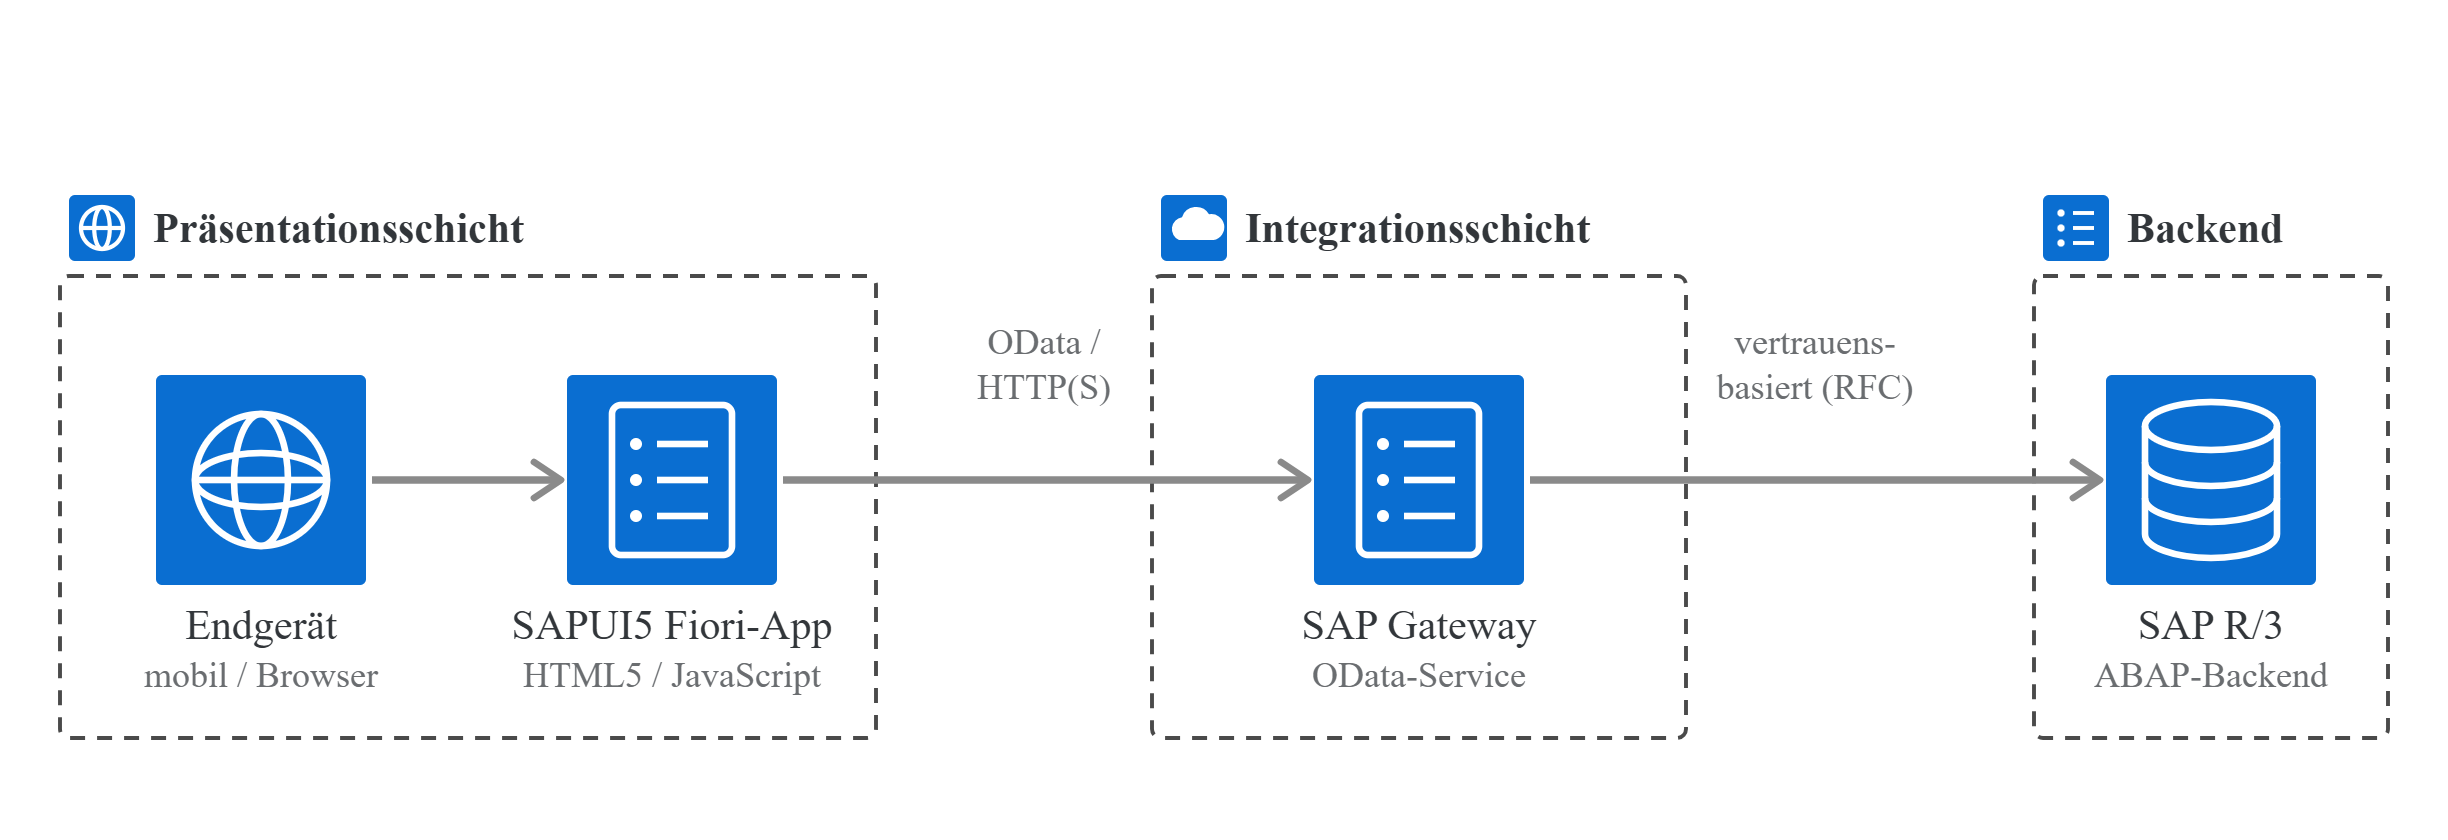
\includegraphics[width=\textwidth]{graphics/sap-fiori-architektur.png}
  \caption{Architektur einer SAPUI5-basierten Fiori-Anwendung}
  \label{abb:fiori-architektur}
\end{figure}


Neben dieser Architektur unterscheidet SAP drei Typen von Fiori-Anwendungen:
transaktionale Anwendungen, Fact-Sheet-Anwendungen und analytische
Anwendungen.\footcite[Vgl.][S.~7]{szirtes_rivlin_2016} Transaktionale Anwendungen
dienen dem aufgabenbezogenen Zugriff und ermöglichen das Ausführen von
Geschäftsvorgängen wie dem Anlegen und Bearbeiten von Belegen.\footcite[Vgl.][S.~16]{mathew_2015}
Die untersuchte Anwendung zur Dokumentation von Instandhaltungsvorgängen lässt sich
als transaktionale Fiori-Anwendung einordnen. Ihre konkrete Ausgestaltung in Form von
Funktionsumfang, Oberflächenaufbau und Nutzungskontext wird im folgenden
Kapitel~\ref{section:untersuchungsgegenstand} beschrieben.

\section{Untersuchungsgegenstand und Nutzungskontext}
\label{section:untersuchungsgegenstand}
Die im vorangegangenen Kapitel als transaktionale Anwendung eingeordnete Fiori-App »Meldung -- Foto aufnehmen« bildet den 
Untersuchungsgegenstand der vorliegenden Arbeit. Im Folgenden wird ihre konkrete Ausgestaltung beschrieben. Zunächst werden Zweck, 
Funktionsumfang, der zugrunde liegende Arbeitsablauf sowie die technische Einbettung der Anwendung dargestellt. Anschließend wird ihr 
Nutzungskontext erläutert, da die Gebrauchstauglichkeit eines interaktiven Systems stets nur in Bezug auf einen konkreten 
Verwendungszusammenhang bestimmt werden kann (vgl. Kapitel~\ref{section:usability}). Die Beschreibung von Untersuchungsgegenstand und 
Nutzungskontext bildet damit den Bewertungsrahmen für die heuristische Evaluation in Kapitel~\ref{chapter:kapitel4}.

\subsection{Untersuchungsgegenstand}

Bei der Anwendung »Meldung -- Foto aufnehmen« handelt es sich um eine SAPUI5-basierte Fiori-Anwendung, deren Aufgabe die fotografische 
Dokumentation von Instandhaltungsvorgängen ist. Ihr Zweck besteht darin, Fotos zu einer bestehenden Instandhaltungsmeldung aufzunehmen 
oder von einem Endgerät hochzuladen und diese eindeutig der jeweiligen Meldungsnummer zuzuordnen. Auf diese Weise wird eine strukturierte 
Bilddokumentation ermöglicht, die im weiteren Instandhaltungsprozess nachvollziehbar bleibt.\footnote{Vgl. Woodward L'Orange GmbH 2026, S.~5. Als firmeninterne Dokumentation wird diese Quelle nicht in den Anhang aufgenommen, kann jedoch auf Anfrage zur Begutachtung zur Verfügung gestellt werden.} Als 
Bezugsobjekt der Dokumentation dient dabei die Meldung des SAP-Moduls PM, die den zentralen Beleg zur Erfassung eines 
Instandhaltungssachverhalts bildet (vgl. Kapitel~\ref{section:Instandhaltungsprozesse}).
Der Funktionsumfang der Anwendung ist auf diesen Dokumentationszweck zugeschnitten und folgt einem festen Bearbeitungsablauf. 
Den Einstieg bildet die Auswahl einer Meldung über eine Suchhilfe, da eine freie manuelle Eingabe der Meldungsnummer nicht vorgesehen 
ist. Zur Eingrenzung des Meldungsbestands stehen Filterkriterien für Kostenstelle, Equipment, Technischer Platz, Meldungsart und 
Erstellungsdatum, sowie eine Freitextsuche über Meldungsnummer und Kurztext zur Verfügung (siehe Abb.~\ref{fig:meldungsauswahl}).\footcite[Vgl.][S.~8~ff.]{woodward2026doku}

\begin{figure}[htbp]
    \centering
    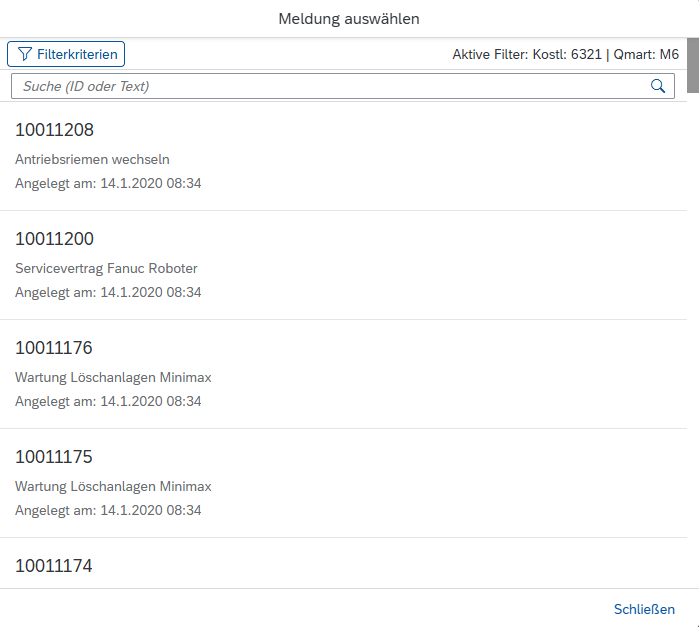
\includegraphics[width=0.7\textwidth]{graphics/meldungsauswahl.png}
    \caption{Dialog zur Meldungsauswahl in der Anwendung}
    \label{fig:meldungsauswahl}
\end{figure}

Nach Auswahl einer Meldung zeigt die Anwendung deren wesentliche Stammdaten in einem Detailbereich an, der dem Benutzer als Prüfhilfe zur 
Bestätigung der korrekten Zuordnung dient.\footcite[Vgl.][S.~15]{woodward2026doku} Erst nach Auswahl einer gültigen Meldung werden die 
Funktionen zur Fotoerfassung freigeschaltet. Dadurch wird verhindert, dass Bilder ohne Bezug zu einer Meldung erfasst 
werden (siehe Abb.~\ref{fig:hauptansicht}).\footcite[Vgl.][S.~16]{woodward2026doku}

\begin{figure}[htbp]
    \centering
    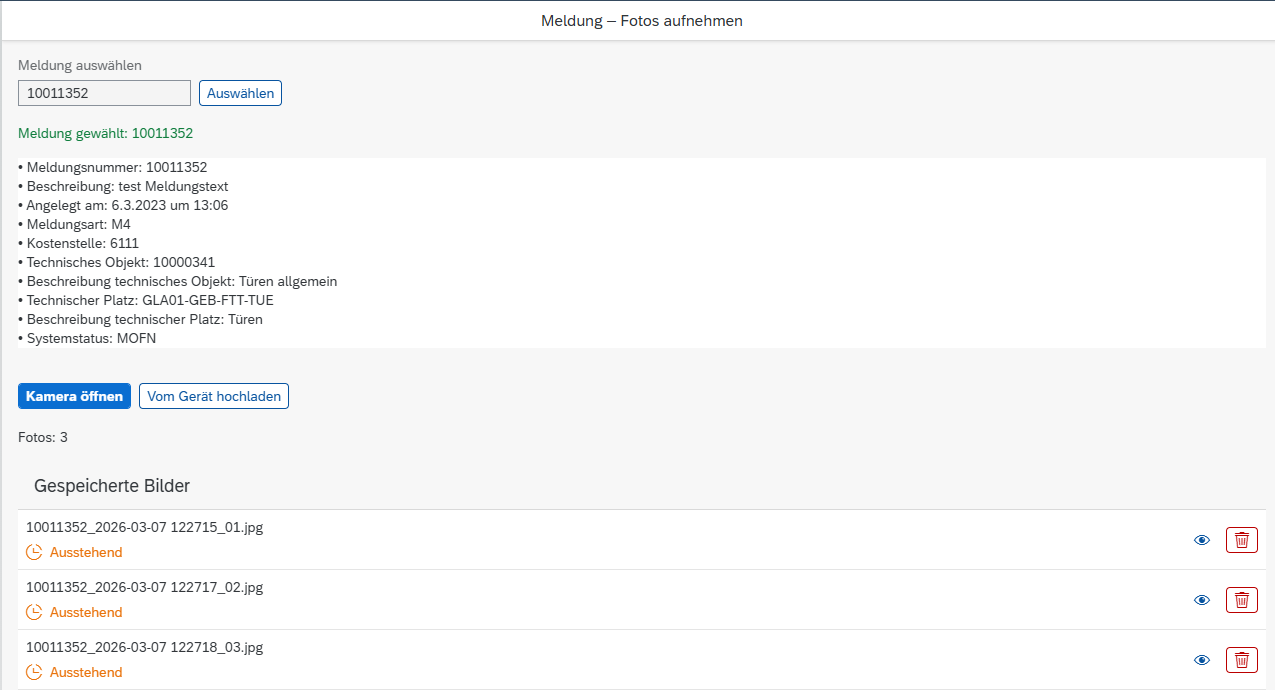
\includegraphics[width=0.7\textwidth]{graphics/hauptansicht.png}
    \caption{Hauptansicht mit Meldungsdetails und freigeschalteten Erfassungsfunktionen}
    \label{fig:hauptansicht}
\end{figure}

Die eigentliche Bilderfassung erfolgt auf zwei Wegen. Über die Gerätekamera nimmt der Benutzer ein Foto auf, das zunächst in einer 
Vorschau zur Kontrolle angezeigt und anschließend übernommen oder verworfen wird (siehe Abb.~\ref{fig:kameradialog}).  

\begin{figure}[htbp]
    \centering
    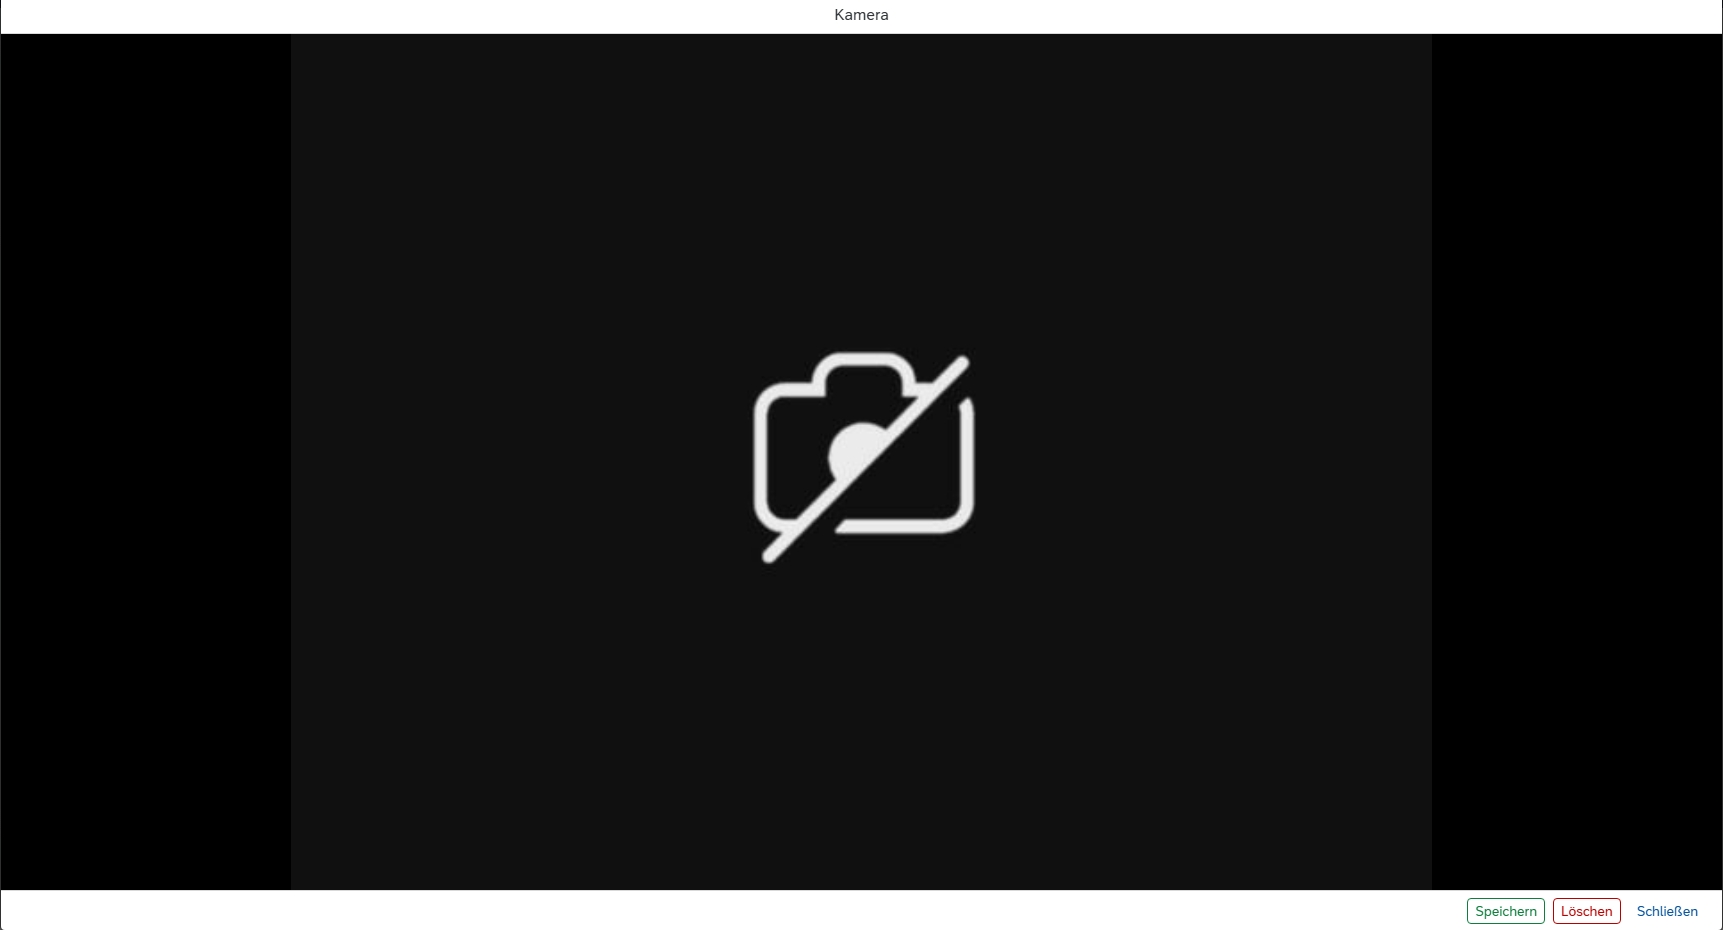
\includegraphics[width=0.7\textwidth]{graphics/kameradialog.jpeg}
    \caption{Kameradialog im Vorschau-Modus zur Kontrolle der Fotoaufnahme}
    \label{fig:kameradialog}
\end{figure}

Alternativ können bereits vorhandene Bilddateien vom 
Endgerät hochgeladen werden.\footcite[Vgl.][S.~16~ff.]{woodward2026doku} Pro Meldung ist die Erfassung auf maximal acht Fotos begrenzt. 
Die übernommenen Bilder werden in einer Fotoliste angezeigt und systematisch benannt, wobei sich der Dateiname aus der Meldungsnummer 
und einer fortlaufenden Nummer zusammensetzt.\footcite[Vgl.][S.~20~f.]{woodward2026doku}
Technologisch ist die Anwendung in die bestehende SAP-Systemlandschaft eingebettet. Die zur Meldungsauswahl benötigten Daten bezieht 
die Anwendung über OData-Services, die über das SAP Gateway bereitgestellt und an das SAP-R/3-Backend angebunden sind. Die Anwendung 
greift somit auf einen klassischen Releasestand zu und nicht auf eine S/4HANA-Umgebung.
Der Aufruf der Anwendung erfolgt browserbasiert auf dem mobilen Endgerät. Eine Besonderheit betrifft die Ablage der erfassten Bilder.
Diese werden nicht als Dokumente innerhalb des SAP-Systems gespeichert, sondern in einem je Meldung angelegten Ordner auf einem 
Fileserver abgelegt. In SAP wird lediglich ein Verweis auf diesen Ablageort hinterlegt, der in der Transaktion IW22 unter den Ablagen 
aufgerufen werden kann. Auf diese Weise bleibt die dateibasierte Bildablage fachlich an die Meldung 
gekoppelt.\footcite[Vgl.][S.~21~f.]{woodward2026doku}
Aus dieser Zweckbestimmung ergibt sich zugleich eine bewusste Abgrenzung des Funktionsumfangs. Die Anwendung dient ausschließlich der 
Fotodokumentation zu bereits bestehenden Meldungen und ermöglicht daher weder das Anlegen noch das Bearbeiten von Meldungen und verändert 
keine Meldungsdaten im SAP-System. Ihr Leistungsumfang ist damit klar auf die Erfassung, Zuordnung und Ablage von Bildern beschränkt.

\subsection{Nutzungskontext}

Die Gebrauchstauglichkeit eines interaktiven Systems lässt sich nur in Bezug auf einen konkreten Nutzungskontext beurteilen, der sich 
nach ISO 9241-11 aus den Benutzern, ihren Arbeitsaufgaben, den eingesetzten Arbeitsmitteln sowie der physischen und sozialen Umgebung 
zusammensetzt (vgl. Kapitel~\ref{section:usability}). Im Folgenden wird dieser Nutzungskontext für die untersuchte Anwendung beschrieben, 
um den Bewertungsmaßstab für die heuristische Evaluation festzulegen.
Die Anwendung richtet sich an die Mitarbeiterinnen und Mitarbeiter 
der Instandhaltung, die unmittelbar vor Ort an den Maschinen tätig sind und die App zur Dokumentation von Defekten einsetzen. Die 
Nutzergruppe umfasst etwa 20 Personen.\footnote{Vgl. Gespräch mit Kaiser 2026, Anhang~\ref{anhang:gespraech}.} 
Kennzeichnend für diese Gruppe ist, dass ihre Tätigkeit handwerklich geprägt ist und sie nur in geringem Umfang mit SAP in 
Berührung kommt. Ihr Zugriff beschränkt sich auf das Einsehen von Meldungen, während das Anlegen oder Bearbeiten von Meldungen nicht zu 
ihren Aufgaben zählt. Die in den Meldungen verwendeten SAP-spezifischen Begriffe und Schlüssel sind den Nutzenden in der Regel nicht 
geläufig.\footnote{Vgl. Gespräch mit Kaiser 2026, Anhang~\ref{anhang:gespraech}.} Die Anwendung wird in 
deutscher Sprache genutzt, eine englische Sprachfassung existiert aufgrund des US-amerikanischen Mutterkonzerns Woodward, bildet jedoch 
nicht den Gegenstand der vorliegenden Untersuchung.
Der Arbeitsumfang besteht in der fotografischen Dokumentation von Defekten, die im Rahmen der Instandhaltung festgestellt werden und 
von routinemäßigen Arbeiten abweichen. Die Fotos werden bereits während des Feststellens des Defekts aufgenommen und dienen der späteren 
Schadensanalyse. Die Nutzung der Anwendung ist nicht verbindlich vorgeschrieben, sondern liegt im Ermessen der einzelnen Mitarbeitenden.

Eingeführt wurde sie im Auftrag des Meisters der Instandhaltung.\footnote{Vgl. Gespräch mit Kaiser 2026, Anhang~\ref{anhang:gespraech}.} 
Über die gesamte Gruppe betrachtet kommt die Anwendung täglich zum Einsatz, von der einzelnen 
Person wird sie hingegen nur etwa zweimal wöchentlich verwendet. Aus dieser Nutzungsfrequenz folgt, dass die Anwendung für die einzelnen 
Nutzenden kein routinemäßig eingeübtes Werkzeug darstellt, sondern eher gelegentlich bedient wird.\footnote{Vgl. Gespräch mit Kaiser 2026, Anhang~\ref{anhang:gespraech}.}
Als Arbeitsmittel dient ein dienstliches Smartphone, auf dem die Anwendung browserbasiert aufgerufen wird. Die Datenverbindung erfolgt 
über das \ac{WLAN} des Standorts. Die Nutzung findet in der Produktionshalle unmittelbar an den Maschinen statt und ist dort durch Lärm, 
Schmutz, Ölrückstände und beengte Platzverhältnisse geprägt. Schutzausrüstung in Form von Schutzbrillen gehört zur üblichen 
Arbeitssituation und je nach Art des Defekts werden zudem zeitweise Handschuhe getragen, die die Bedienung des Touchscreens situativ 
erschweren können. Für die Dokumentation selbst steht den Mitarbeitenden ausreichend Zeit zur 
Verfügung.\footnote{Vgl. Gespräch mit Kaiser 2026, Anhang~\ref{anhang:gespraech}.}
Der beschriebene Nutzungskontext bildet den Maßstab, an dem die Gebrauchstauglichkeit der Anwendung im folgenden Kapitel zu messen ist. 
Insbesondere die Kombination aus geringer SAP-Vertrautheit der Nutzenden, der nur gelegentlichen Verwendung und den anspruchsvollen 
Umgebungsbedingungen lässt erwarten, dass an die Verständlichkeit und die Bedienbarkeit der Anwendung besondere Anforderungen zu stellen 
sind. Vor diesem Hintergrund werden die Interaktionsprinzipien der ISO 9241-110 im folgenden Kapitel zu einem Kriterienkatalog 
operationalisiert und auf die Anwendung angewendet.


\chapter{Heuristische Evaluation der Anwendung}
\label{chapter:kapitel4}
Durchführung der eigentlichen Evaluation auf Basis eines operationalisierten
Kriterienkatalogs, Dokumentation der Befunde mit Schweregradbewertung und
Ableitung von Optimierungspotenzialen.

\section{Untersuchungsdesign und Operationalisierung}
\label{section:untersuchungsdesign}

Die Untersuchung erfolgt als heuristische Evaluation in Form einer
Experteninspektion.
Statt die Anwendung durch Endnutzer erproben zu lassen, prüft der Evaluator sie
systematisch gegen einen zuvor festgelegten
Kriterienkatalog.\footcite[Vgl.][S.~254 f.]{nielsen1990heuristic}
Dazu durchläuft er die für die Bilddokumentation relevanten Aufgabenpfade
mehrfach und gleicht die einzelnen Dialogelemente mit den Prüfkriterien ab.
Der Inspektionsumfang beschränkt sich auf die in
Kapitel~\ref{section:untersuchungsgegenstand} beschriebenen Funktionen.
Dass der Verfasser die identifizierten Abweichungen im Anschluss selbst als
Entwickler behebt, ist eine methodische Einschränkung und wird in
Kapitel~\ref{grenzen} reflektiert.

Als Bewertungsmaßstab dienen die sieben Interaktionsprinzipien der ISO~9241-110
(Kapitel~\ref{grundsaetzeISO}).
Da sie abstrakt formuliert sind, werden sie für die Evaluation operationalisiert,
also in überprüfbare Prüfkriterien überführt.
Grundlage ist die normeigene Anwendungstabelle (Tabelle~A.1), die zu jedem
Prinzip konkrete Gestaltungsempfehlungen
aufführt.\footcite[Vgl.][Tabelle~A.1]{DIN_ISO_9241-110:2020}
Jede Empfehlung wird zunächst auf ihre Anwendbarkeit im vorliegenden
Nutzungskontext geprüft.
Nicht anwendbare Empfehlungen werden ausgeschlossen, wie es die Norm vorsieht.
Von den 64 Einzelempfehlungen entfallen so 22.
Die verbleibenden 42 werden zu 41 aufgabenbezogenen Prüffragen operationalisiert,
die sich mit \enquote{erfüllt} oder \enquote{Abweichung} beantworten lassen,
wobei Kriterium~7.4 zwei Empfehlungen zur Vertrauenswürdigkeit
bündelt.\footcite[Vgl.][Tabelle~A.1]{DIN_ISO_9241-110:2020}
Der Kriterienkatalog ist in Anhang~\ref{anhang:kriterienkatalog} vollständig
dokumentiert und lässt sich grundsätzlich auf vergleichbare mobile
SAP-Fiori-Anwendungen übertragen.

Jede festgestellte Abweichung wird als Usability-Problem dokumentiert, dem
verletzten Prinzip zugeordnet und nach \ac{SG} eingestuft.
Dafür dient die fünfstufige Skala nach Nielsen, die von
\enquote{kein Usability-Problem} (0) bis \enquote{Usability-Katastrophe} (4)
reicht.\footcite[Vgl.][S.~47]{nielsen1994heuristic}
Die Einstufung richtet sich nach Häufigkeit, Schwere der Auswirkung und
Persistenz des Problems.\footcite[Vgl.][S.~47]{nielsen1994heuristic}

\begin{table}[htbp]
\centering
\caption[Schweregradskala nach Nielsen]{Schweregradskala nach
Nielsen\footcite[Mit Änderungen entnommen aus:][S.~47]{nielsen1994heuristic}}
\label{tab:schweregrade}
\begin{tabularx}{0.98\textwidth}{|c|>{\RaggedRight}X|}
\hline
\textbf{Grad} & \textbf{Bedeutung} \\\hline
0 & Kein Usability-Problem \\\hline
1 & Kosmetisches Problem - Behebung nur bei freier Kapazität \\\hline
2 & Geringfügiges Problem - niedrige Behebungspriorität \\\hline
3 & Schwerwiegendes Problem - hohe Behebungspriorität \\\hline
4 & Usability-Katastrophe - Behebung vor Auslieferung zwingend \\\hline
\end{tabularx}
\end{table}

Um die Forschungsfrage nach dem \emph{Inwieweit} der Erfüllung zu beantworten,
wird je Prinzip ein Erfüllungsgrad aus den zugehörigen Prüfkriterien abgeleitet.
Ein Prinzip gilt als \emph{erfüllt}, wenn keine oder nur kosmetische Abweichungen
(Schweregrad~$\leq 1$) vorliegen, als \emph{teilweise erfüllt} bei Abweichungen
bis Schweregrad~3 und als \emph{nicht erfüllt}, sobald eine Abweichung des
Schweregrades~4 oder mehrere des Schweregrades~3 auftreten.
Diese Zuordnung macht die Bewertung in Kapitel~\ref{section:ergebnisse}
nachvollziehbar und vergleichbar.


\section{Ergebnisse und Schweregradbewertung}
\label{section:ergebnisse}

Geprüft wurden die 41 im Nutzungskontext anwendbaren Kriterien des
Kriterienkatalogs.
Bei 11 davon wurde eine Abweichung festgestellt, 30 waren erfüllt.
Die Abweichungen verteilen sich auf zwei Befunde des Schweregrades~1, fünf des
Schweregrades~2 und vier des Schweregrades~3.
Eine Usability-Katastrophe (Schweregrad~4) trat nicht auf
(vgl. Tabelle~\ref{tab:schweregrade}).
Die Darstellung erfolgt prinzipienweise.
Je Prinzip werden zunächst die erfüllten Kriterien genannt, dann die Abweichungen
einzeln, jeweils mit verletzter Normanforderung, konkreter Beobachtung und
Begründung der Schweregradeinstufung.
Abschließend wird der Erfüllungsgrad nach der in
Kapitel~\ref{section:untersuchungsdesign} festgelegten Logik bestimmt.\\
\textbf{Prinzip 1 -- Aufgabenangemessenheit:}
Für die Aufgabenangemessenheit wurden fünf Kriterien geprüft, keines wies eine
Abweichung auf.
Die Anwendung macht ihren Zweck, die fotografische Dokumentation zu einer
bestehenden Instandhaltungsmeldung, hinreichend deutlich (Kriterium~1.1), und in
jedem Schritt des Ablaufs, von der Meldungsauswahl über die Fotoaufnahme bis zur
Fotoverwaltung, stehen die erforderlichen Steuerelemente und Informationen bereit
(Kriterium~1.2).
Da der Funktionsumfang bewusst eng auf den Dokumentationszweck zugeschnitten ist
(vgl. Kapitel~\ref{section:untersuchungsgegenstand}), enthält die Anwendung
nichts, was von der Aufgabe ablenkt (Kriterium~1.3).
Sie bietet Vorbelegungen dort, wo sie zweckmäßig sind, und vermeidet solche, die
eine Fehlzuordnung der Fotos begünstigen könnten (Kriterien~1.4 und~1.5).
Das Prinzip gilt als \emph{erfüllt}.\\
\textbf{Prinzip 2 -- Selbstbeschreibungsfähigkeit:}
Von sieben Kriterien waren vier erfüllt.
Die erforderlichen Steuerelemente lassen sich zuverlässig auffinden
(Kriterium~2.2), der Bearbeitungsfortschritt ist über die Zahl erfasster Fotos
und den Bezug zur gewählten Meldung erkennbar (Kriterium~2.5), das Übernehmen
oder Verwerfen eines Fotos wird zurückgemeldet (Kriterium~2.6), und es ist
erkennbar, dass zunächst eine Meldung auszuwählen ist, bevor die Fotofunktionen
bereitstehen (Kriterium~2.7).
Drei Kriterien wiesen Abweichungen auf.
\newpage

Nach der Norm soll ein System eindeutig anzeigen, wo sich Benutzende befinden,
welche Handlungen möglich und welche Einstellungen wirksam
sind.\footcite[Vgl.][Abschnitt~5.2.2.2]{DIN_ISO_9241-110:2020}
In der Meldungssuche ist der wirksame Zustand nur eingeschränkt erkennbar.
Welche Filter aktiv sind, steht abseits im oberen rechten Fensterbereich und ist
leicht zu übersehen.
An einzelnen Bedienschritten fehlen zudem Hinweise auf die möglichen Aktionen
(Kriterium~2.1).
Da die Meldungssuche den Einstieg in jeden Vorgang bildet, tritt der Mangel
regelmäßig auf.
Seine Auswirkung bleibt moderat, weil ein übersehener Filter zu einer leeren oder
unvollständigen Trefferliste führt, den Vorgang aber nicht blockiert.
Die Abweichung wird als Schweregrad~2 eingestuft.

Interaktive Elemente sollen klar als solche erkennbar
sein.\footcite[Vgl.][Abschnitt~5.2.2.4]{DIN_ISO_9241-110:2020}
Die Buttons sind jedoch uneinheitlich gestaltet.
Einer erscheint blau gefüllt mit weißer Fettschrift, ein anderer nur blau
umrandet mit dünner blauer Schrift, sodass ihr Interaktionscharakter weniger
unmittelbar erschließbar ist (Kriterium~2.3).
Da die Schaltflächen bedienbar bleiben und die Aufgabenerledigung nicht behindert
wird, gilt der Befund als kosmetische Abweichung mit Schweregrad~1.

Informationen sollen in einem den Benutzenden vertrauten Vokabular
erscheinen.\footcite[Vgl.][Abschnitt~5.2.2.5]{DIN_ISO_9241-110:2020}
Die Meldungsart wird jedoch allein als SAP-internes Kürzel wie \enquote{M1}
angezeigt, ohne Klartext (Kriterium~2.4).
Für die handwerklich geprägte, mit SAP wenig vertraute Nutzergruppe
(vgl. Kapitel~\ref{section:untersuchungsgegenstand}) bleibt damit unklar, welche
Meldungsart sich hinter dem Kürzel verbirgt.
Das Kürzel erscheint bei jeder Meldungsauswahl und betrifft mit der
Identifikation der richtigen Meldung einen zentralen Schritt.
Da sich das Vokabular bei nur etwa zweimal wöchentlicher Nutzung kaum einprägt,
wirkt der Mangel dauerhaft und kann eine Fehlauswahl begünstigen.
Weil die angezeigten Stammdaten eine Fehlauswahl aber erkennen und korrigieren
lassen (vgl. Kriterium~6.7), bleibt die Auswirkung begrenzt und die Abweichung
wird als Schweregrad~2 eingestuft.
Mit den Kriterien~2.1 und~2.4 liegen zwei Abweichungen des Schweregrades~2 vor.
Das Prinzip gilt als \emph{teilweise erfüllt}.\\
\textbf{Prinzip 3 -- Erwartungskonformität:}
Von sieben Kriterien waren fünf erfüllt.
Die Ablaufschritte entsprechen dem Aufgabenverständnis der
Instandhaltungsmitarbeitenden (Kriterium~3.1), unmittelbare Handlungen wie das
Auslösen der Kamera werden sofort zurückgemeldet (Kriterium~3.2), Elemente
unterschiedlichen Zwecks sind erkennbar abgegrenzt (Kriterium~3.5), auf
Änderungen angeschlossener Ressourcen reagiert die Anwendung angemessen
(Kriterium~3.6), und die Inhalte werden auf der Smartphone-Anzeige passend
dargestellt (Kriterium~3.7).
Zwei Kriterien wiesen Abweichungen auf.

Bei erwartbar langen Reaktionszeiten soll eine Fortschrittsinformation ausgegeben
werden.\footcite[Vgl.][Abschnitt~5.3.2.4]{DIN_ISO_9241-110:2020}
Beim Laden der Meldungsliste oder beim Hochladen von Fotos über das Standort-WLAN
bleibt eine solche Anzeige jedoch aus, sodass nicht erkennbar ist, ob das System
noch arbeitet (Kriterium~3.3).
Das kann Benutzende dazu verleiten, eine Aktion für fehlgeschlagen zu halten und
zu wiederholen.
Da die Aufgabe erschwert, aber nicht verhindert wird, gilt die Abweichung als
Schweregrad~2.

Für die Darstellung sollen den Benutzenden vertraute sprachliche Konventionen
verwendet werden.\footcite[Vgl.][Abschnitt~5.3.3.1]{DIN_ISO_9241-110:2020}
Deutsche und englische Oberflächentexte wechseln sich jedoch ohne erkennbare
Systematik ab (Kriterium~3.4), was der Erwartung einer durchgängig
deutschsprachigen Oberfläche
(vgl. Kapitel~\ref{section:untersuchungsgegenstand}) widerspricht.
Da die Sprachmischung die gesamte Anwendung durchzieht und das Verständnis der
überwiegend nicht englischsprachig arbeitenden Nutzergruppe spürbar erschwert,
wird die Abweichung als Schweregrad~3 eingestuft.
Damit gilt das Prinzip als \emph{teilweise erfüllt}.\\
\textbf{Prinzip 4 -- Erlernbarkeit:}
Alle vier geprüften Kriterien waren erfüllt.
Die Anwendung unterstützt Benutzende dabei, die nötigen Funktionen selbstständig
zu entdecken und zielführend zu nutzen (Kriterium~4.1).
Sie lässt sich gefahrlos erkunden, da jede Aufnahme vor der Übernahme in einer
Vorschau geprüft und ohne Folgen verworfen werden kann (Kriterium~4.2).
Für das Auffinden der richtigen Meldung stehen mit Filterkriterien und
Freitextsuche alternative Wege bereit (Kriterium~4.3), und Rückmeldungen lassen
die Folgen der eigenen Aktionen erkennen (Kriterium~4.4).
Das Prinzip gilt als \emph{erfüllt}.\\
\textbf{Prinzip 5 -- Steuerbarkeit:}
Alle vier geprüften Kriterien waren erfüllt.
Benutzende können den Vorgang jederzeit unterbrechen (Kriterium~5.1) und
fortsetzen, ohne Meldungsauswahl oder erfasste Fotos zu verlieren (Kriterium~5.2).
Für die Bilderfassung stehen mit Gerätekamera und Datei-Upload zwei Wege zur
Verfügung (Kriterium~5.3), und zumindest die letzte Aktion lässt sich rückgängig
machen, indem ein Foto verworfen oder wieder entfernt wird (Kriterium~5.4).
Das Prinzip gilt als \emph{erfüllt}.\\
\textbf{Prinzip 6 -- Robustheit gegen Benutzungsfehler:}
Mit fünf Abweichungen bei zehn Kriterien wies dieses Prinzip die meisten Befunde
auf.
Erfüllt waren die Vermeidung erneuter Eingabe bereits vorhandener Informationen
(Kriterium~6.1), die Meldungsauswahl über eine Suchhilfe nach dem Prinzip der
Wiedererkennung (Kriterium~6.2), die Sicherung erfasster Fotos gegen Verlust
durch System- oder Verbindungsfehler (Kriterium~6.4), die Unterstützung beim
Erkennen einer Fehlauswahl über die angezeigten Stammdaten (Kriterium~6.7) sowie
der geringe Korrekturaufwand (Kriterium~6.10).
Die fünf Abweichungen betreffen Fehlervermeidung, Fehlererkennung und
Fehlerbehebung.

Es sollen nur aktuell gültige Auswahlmöglichkeiten zugelassen
werden.\footcite[Vgl.][Abschnitt~5.6.2.3]{DIN_ISO_9241-110:2020}
In der Meldungssuche lassen sich jedoch einander ausschließende Filter
kombinieren.
Nach Auswahl einer Kostenstelle (etwa KST6336) bleibt eine Maschine (etwa
Index G-550) wählbar, die dieser Kostenstelle nicht zugeordnet ist, sodass die
Suche zwangsläufig ohne Ergebnis bleibt (Kriterium~6.3).
Der Fall tritt nur bei bestimmten Kombinationen auf und lässt sich durch Anpassen
der Filter auflösen.
Die Abweichung wird als Schweregrad~2 eingestuft.

Eingabefehler sollen bereits vor der Weiterverarbeitung erkannt
werden.\footcite[Vgl.][Abschnitt~5.6.2.5]{DIN_ISO_9241-110:2020}
Beim Hochladen einer Datei ungeeigneten Formats bleibt jede Rückmeldung aus.
Die Datei wird ohne Hinweis verworfen (Kriterium~6.5).
Benutzende gehen dann davon aus, das Foto sei erfasst, während es tatsächlich
fehlt, sodass eine Lücke in der Dokumentation entsteht, die womöglich erst bei
der späteren Schadensanalyse auffällt.
Wegen dieser gravierenden und ohne Rückmeldung nicht erkennbaren Auswirkung wird
die Abweichung als Schweregrad~3 eingestuft.

Vor Handlungen mit schwerwiegenden Auswirkungen soll das System eine Bestätigung
einholen.\footcite[Vgl.][Abschnitt~5.6.2.6]{DIN_ISO_9241-110:2020}
Ein bereits erfasstes Foto wird jedoch mit einem einzigen Klick und ohne Rückfrage
gelöscht (Kriterium~6.6).
Da es sich vor Ort nicht ohne Weiteres erneut aufnehmen lässt, der dokumentierte
Zustand am Objekt besteht dann möglicherweise nicht mehr, kann eine Fehlbedienung
unmittelbar zu unwiederbringlichem Datenverlust führen.
Der Verlust setzt zwar eine Fehlbedienung voraus und tritt selten auf.
Wegen der Unumkehrbarkeit wird die Abweichung aber nicht als kosmetisch, sondern
als Schweregrad~2 eingestuft.

Die beiden verbleibenden Abweichungen gehen auf dasselbe Fehlverhalten bei
Fehlermeldungen zurück.
Bei manchen Fehlern erscheint zwar ein Popup, es enthält aber nur den Hinweis
\enquote{Fehlermeldung kann nicht geladen werden} statt des eigentlichen
Fehlertextes.
Damit ist die Anforderung, präzise und ohne Fachkenntnisse verständliche
Fehlermeldungen
auszugeben,\footcite[Vgl.][Abschnitt~5.6.4.2]{DIN_ISO_9241-110:2020} nicht erfüllt
(Kriterium~6.8).
Das Popup zeigt an, dass ein Problem vorliegt, benennt aber weder Art noch
Ursache, sodass Benutzende genau in der Störungssituation ohne verwertbare
Rückmeldung dastehen.
Wegen dieser in jedem Fehlerfall auftretenden Intransparenz wird der Befund als
Schweregrad~3 eingestuft.
Zugleich soll eine Fehlermeldung konstruktive Erläuterungen zu ihrer Behebung
liefern.\footcite[Vgl.][Abschnitt~5.6.4.3]{DIN_ISO_9241-110:2020}
Die Meldung nennt jedoch keine Handlungsanweisung, mit der Benutzende den Fehler
selbst beheben könnten (Kriterium~6.9).
Da sie ohne eine solche Anweisung den Vorgang nicht fortsetzen können und auf
fremde Unterstützung angewiesen sind, wird auch dieser Befund als Schweregrad~3
eingestuft.
Mit den Kriterien~6.5, 6.8 und~6.9 liegen drei Abweichungen des Schweregrades~3
vor.
Das Prinzip gilt als \emph{nicht erfüllt}.\\
\textbf{Prinzip 7 -- Benutzerbindung:}
Von vier Kriterien waren drei erfüllt.
Die Anwendung bestätigt die erfolgreiche Erfassung und Zuordnung der Fotos und
macht erkennbar, dass keine offenen Schritte verbleiben (Kriterium~7.1).
Sie benennt die Fotos automatisch aus Meldungsnummer und fortlaufender Nummer und
ordnet sie der Meldung zu (Kriterium~7.2), und die nachvollziehbare Ablage
rechtfertigt das Vertrauen in eine korrekte und zuverlässige Speicherung
(Kriterium~7.4).
Eine Abweichung wurde festgestellt.

Die Anwendung soll keine unverhältnismäßigen Anforderungen an die Benutzenden
stellen.\footcite[Vgl.][Abschnitt~5.7.2.7]{DIN_ISO_9241-110:2020}
Die Bedienung ist jedoch nicht auf die erschwerten Bedingungen in der Produktion
ausgelegt.
Insbesondere fehlt eine Anpassung an die Bedienung mit Handschuhen, die situativ
getragen werden (Kriterium~7.3,
vgl. Kapitel~\ref{section:untersuchungsgegenstand}).
Da die Handschuhe nur zeitweise getragen werden, sich die Erschwernis durch
kurzes Ablegen umgehen lässt und für die Dokumentation genügend Zeit bleibt, gilt
die Abweichung als kosmetischer Mangel mit Schweregrad~1.
Damit gilt das Prinzip als \emph{erfüllt}.

\bigskip
Tabelle~\ref{tab:erfuellungsgrad} fasst die Bewertung zusammen.
Von den sieben Prinzipien sind vier erfüllt, zwei teilweise erfüllt und eines,
die Robustheit gegen Benutzungsfehler, nicht erfüllt.
Die Abweichungen konzentrieren sich auf Selbstbeschreibungsfähigkeit,
Erwartungskonformität und vor allem Robustheit gegen Benutzungsfehler, während
die aufgabenbezogenen Prinzipien Aufgabenangemessenheit, Erlernbarkeit und
Steuerbarkeit vollständig erfüllt sind.

\begin{table}[htbp]
\centering
\caption{Erfüllungsgrad der Interaktionsprinzipien im Überblick}
\label{tab:erfuellungsgrad}
\begin{tabularx}{\textwidth}{|>{\RaggedRight}X|c|c|c|c|}
\hline
\textbf{Prinzip} & \textbf{Geprüft} & \textbf{Abw.} & \textbf{Max. SG} & \textbf{Erfüllungsgrad} \\\hline
1 Aufgabenangemessenheit & 5 & 0 & 0 & erfüllt \\\hline
2 Selbstbeschreibungsfähigkeit & 7 & 3 & 2 & teilweise erfüllt \\\hline
3 Erwartungskonformität & 7 & 2 & 3 & teilweise erfüllt \\\hline
4 Erlernbarkeit & 4 & 0 & 0 & erfüllt \\\hline
5 Steuerbarkeit & 4 & 0 & 0 & erfüllt \\\hline
6 Robustheit gegen Benutzungsfehler & 10 & 5 & 3 & nicht erfüllt \\\hline
7 Benutzerbindung & 4 & 1 & 1 & erfüllt \\\hline
\end{tabularx}
\end{table}


\section{Optimierungspotenziale}
\label{section:optimierungspotenziale}

Aus den in Kapitel~\ref{section:ergebnisse} dokumentierten Abweichungen lassen
sich konkrete Optimierungspotenziale ableiten, erfüllte Kriterien erfordern keine
Maßnahme.
Die Priorisierung folgt dem Schweregrad, der nach Nielsen unmittelbar den
Behebungsaufwand priorisiert.\footcite[Vgl.][S.~47]{nielsen1994heuristic}
Abweichungen mit gemeinsamer Ursache oder gemeinsamem Themenfeld werden zu einem
Maßnahmenbündel zusammengefasst, das die Priorität seiner schwerwiegendsten
Abweichung erhält.
Bündel mit Schweregrad~3 werden mit hoher, solche mit maximal Schweregrad~2 mit
mittlerer und rein kosmetische Befunde mit niedriger Priorität eingeordnet
(vgl. Tabelle~\ref{tab:optimierung}).

\textbf{Robustheit gegen Benutzungsfehler:}
Der größte Handlungsbedarf besteht beim einzigen nicht erfüllten Prinzip.
Beim Hochladen einer Datei ungeeigneten Formats sollte die Anwendung das Format
prüfen und unmittelbar zurückmelden, statt die Datei unbemerkt zu verwerfen
(Kriterium~6.5).
Das erkennt Eingabefehler vor der
Weiterverarbeitung\footcite[Vgl.][Abschnitt~5.6.2.5]{DIN_ISO_9241-110:2020} und
verhindert unbemerkte Lücken in der Bilddokumentation.
Die bei Ladefehlern ausgegebene Meldung sollte den eigentlichen Fehlertext
zuverlässig anzeigen, ihn zielgruppengerecht formulieren und um eine konkrete
Handlungsanweisung ergänzen, etwa den Hinweis, dass die Meldungsliste nicht
geladen werden konnte, verbunden mit der Empfehlung, den Vorgang erneut zu starten
(Kriterien~6.8 und~6.9).
So entstehen präzise, verständliche Fehlermeldungen mit konstruktiven
Erläuterungen.\footcites[Vgl.][Abschnitt~5.6.4.2]{DIN_ISO_9241-110:2020}[Vgl.][Abschnitt~5.6.4.3]{DIN_ISO_9241-110:2020}
Vor dem Löschen eines erfassten Fotos sollte eine Bestätigung abgefragt werden
(Kriterium~6.6), um unwiederbringlichen Datenverlust durch Fehlbedienung zu
vermeiden.\footcite[Vgl.][Abschnitt~5.6.2.6]{DIN_ISO_9241-110:2020}
Schließlich sollten in der Meldungssuche abhängige Filter so verknüpft werden,
dass nach einer Auswahl nur noch passende Folgewerte erscheinen (Kriterium~6.3).
Das lässt ausschließlich gültige Auswahlmöglichkeiten
zu\footcite[Vgl.][Abschnitt~5.6.2.3]{DIN_ISO_9241-110:2020} und schließt
ergebnislose Kombinationen aus.\\
\textbf{Verständlichkeit von Begriffen und Sprache:}
Ebenfalls hohe Priorität hat die Verständlichkeit für die handwerklich geprägte,
mit SAP wenig vertraute Nutzergruppe
(vgl. Kapitel~\ref{section:untersuchungsgegenstand}).
Die Meldungsart sollte zusätzlich zum internen Kürzel im Klartext erscheinen
(Kriterium~2.4), damit Informationen in vertrautem Vokabular dargestellt
werden,\footcite[Vgl.][Abschnitt~5.2.2.5]{DIN_ISO_9241-110:2020} und die
Oberflächentexte sollten durchgängig deutsch gehalten werden (Kriterium~3.4), um
vertrauten sprachlichen Konventionen zu
entsprechen.\footcite[Vgl.][Abschnitt~5.3.3.1]{DIN_ISO_9241-110:2020}
Beide Maßnahmen senken das Risiko einer Fehlauswahl der Meldung und damit einer
Fehlzuordnung der Fotos.\\
\textbf{Transparenz von Systemzustand und Rückmeldung:}
Mit mittlerer Priorität sollte die Erkennbarkeit des Systemzustands verbessert
werden.
Die aktiven Filter sollten sichtbar und zentral im Suchbereich erscheinen statt
abseits am oberen Fensterrand (Kriterium~2.1), sodass jederzeit erkennbar ist,
welche Einstellungen
wirken.\footcite[Vgl.][Abschnitt~5.2.2.2]{DIN_ISO_9241-110:2020}
Bei länger dauernden Vorgängen wie dem Laden der Meldungsliste oder dem Hochladen
von Fotos sollte eine Warte- oder Fortschrittsanzeige erscheinen (Kriterium~3.3),
damit erkennbar bleibt, dass das System
arbeitet.\footcite[Vgl.][Abschnitt~5.3.2.4]{DIN_ISO_9241-110:2020}\\
\textbf{Konsistenz der Oberflächengestaltung:}
Mit niedriger Priorität empfiehlt sich, die Schaltflächen nach einem einheitlichen
Schema zu gestalten, das primäre und sekundäre Aktionen klar unterscheidet
(Kriterium~2.3), damit ihr Interaktionscharakter unmittelbarer erkennbar
wird.\footcite[Vgl.][Abschnitt~5.2.2.4]{DIN_ISO_9241-110:2020}\\
\textbf{Anpassung an den Einsatzkontext vor Ort:}
Ebenfalls niedrige Priorität hat die Anpassung an die Einsatzbedingungen vor Ort,
insbesondere größere, auch mit Handschuhen sicher bedienbare Bedienelemente
(Kriterium~7.3), um keine unverhältnismäßigen Anforderungen zu
stellen.\footcite[Vgl.][Abschnitt~5.7.2.7]{DIN_ISO_9241-110:2020}

Tabelle~\ref{tab:optimierung} fasst die abgeleiteten Maßnahmen mit
Kriteriumsbezug, Schweregrad und Priorität zusammen.

\begin{table}[htbp]
\centering
\caption{Abgeleitete Optimierungspotenziale im Überblick}
\label{tab:optimierung}
{\footnotesize
\begin{tabularx}{\textwidth}{|c|>{\RaggedRight}X|c|c|}
\hline
\textbf{Krit.} & \textbf{Maßnahme} & \textbf{SG} & \textbf{Priorität} \\\hline
6.5 & Dateiformat prüfen und Upload-Fehler zurückmelden & 3 & hoch \\\hline
6.8 & Fehlertext korrekt anzeigen & 3 & hoch \\\hline
6.9 & Fehlermeldungen mit konkreter Handlungsanweisung versehen & 3 & hoch \\\hline
6.6 & Bestätigungsabfrage vor dem Löschen eines Fotos & 2 & hoch \\\hline
6.3 & Abhängige Filter dynamisch auf gültige Werte einschränken & 2 & hoch \\\hline
3.4 & Oberfläche durchgängig deutschsprachig gestalten & 3 & hoch \\\hline
2.4 & Meldungsart zusätzlich im Klartext anzeigen & 2 & hoch \\\hline
2.1 & Aktive Filter sichtbar und zentral anzeigen & 2 & mittel \\\hline
3.3 & Warte-/Fortschrittsanzeige bei langen Vorgängen & 2 & mittel \\\hline
2.3 & Schaltflächen nach einheitlichem Schema gestalten & 1 & niedrig \\\hline
7.3 & Bedienelemente für Handschuhnutzung vergrößern & 1 & niedrig \\\hline
\end{tabularx}
}
\end{table}

\chapter{Diskussion}
\label{chapter:kapitel5}
Einordnung und Interpretation der Evaluationsergebnisse im Gesamtkontext sowie kritische Reflexion der methodischen Grenzen, 
insbesondere der nachgelagerten Rollenübernahme als Entwickler nach Abschluss der Evaluation.

\section{Interpretation der Befunde im Gesamtkontext}
\label{gesamtkontext}

Von den sieben Interaktionsprinzipien der ISO~9241-110 sind vier vollständig, zwei
teilweise und ein Prinzip nicht erfüllt (vgl. Tabelle~\ref{tab:erfuellungsgrad}).
Über die prinzipienweise Betrachtung in Kapitel~\ref{section:ergebnisse} hinaus
lassen sich die elf Abweichungen zu drei Mustern verdichten.

Ein erstes Muster zeigt sich bei den Kriterien~2.1, 3.3, 6.3, 6.5, 6.6, 6.8 und~6.9.
Sie betreffen ausnahmslos Situationen, in denen die Anwendung auf Fehler, Ausnahmen
oder Rückmeldebedarf reagieren muss, etwa bei nicht erkennbaren aktiven Filtern,
fehlenden Warteinformationen, ungültigen Dateiformaten oder gescheiterten
Ladevorgängen. Die unmittelbar aufgabenbezogenen Prinzipien Aufgabenangemessenheit,
Erlernbarkeit und Steuerbarkeit sind dagegen vollständig erfüllt, was der in
Kapitel~\ref{section:problemstellung} beschriebenen Ausgangslage entspricht, wonach
die Anwendung bislang zwar funktional, jedoch nicht systematisch geprüft wurde.
Mit den Kriterien~6.5, 6.8 und~6.9 sind drei der vier Abweichungen
des Schweregrades~3 genau diesem Muster zuzuordnen.

Ein zweites Muster betrifft die sprachliche Verständlichkeit der Oberfläche. Die
Kriterien~2.4 und~3.4 (Meldungsart als SAP-Kürzel, Sprachmischung) sind mit
Schweregrad~3 beziehungsweise~2 eingestuft. Angesichts des in
Kapitel~\ref{section:untersuchungsgegenstand} beschriebenen Nutzungskontexts,
insbesondere der geringen SAP-Vertrautheit der rund 20 Nutzenden und der nur
zweimal wöchentlichen Nutzungsfrequenz, wiegen diese Befunde schwer. Das
erforderliche Vokabular prägt sich kaum ein, sodass die Mängel strukturell die
gesamte Zielgruppe betreffen.

Ein drittes, gegenläufiges Muster zeigt Kriterium~7.3 (fehlende Anpassung an
Handschuhnutzung). Trotz niedrigstem Schweregrad~1 weist es den unmittelbarsten
Bezug zu den physischen Rahmenbedingungen der Produktionshalle auf. Schweregrad
und Kontextrelevanz eines Befundes fallen demnach nicht notwendig zusammen.

Der aus Tabelle~A.1 der Norm entwickelte Kriterienkatalog
(Kapitel~\ref{section:untersuchungsdesign}) erweist sich damit, trotz der in
Kapitel~\ref{grenzen} diskutierten Einschränkungen, als hinreichend trennscharf.
Er macht sowohl die Erfüllung im Kernablauf als auch gezielte Abweichungen in
Randbereichen sichtbar. Für Woodward L'Orange knüpft dies unmittelbar an die in
Kapitel~\ref{section:problemstellung} beschriebene Ausgangslage an. An die Stelle
einer zuvor fehlenden objektivierbaren Grundlage tritt eine priorisierte Übersicht
identifizierter Schwachstellen (vgl. Tabelle~\ref{tab:optimierung}), wobei die
vier Abweichungen des Schweregrades~3 vorrangig zu adressieren
sind.\footcite[Vgl.][S.~47]{nielsen1994heuristic}

\section{Methodische Grenzen der Untersuchung}
\label{grenzen}

Eine methodische Besonderheit liegt in der Rollenkonstellation des Verfassers. An der
ursprünglichen Entwicklung der Anwendung war er nicht beteiligt und kannte diese zum
Zeitpunkt der Evaluation noch nicht (vgl. Kapitel~\ref{section:untersuchungsdesign}), sodass
das für Inspektionsverfahren relevante Risiko einer Betriebsblindheit gegenüber selbst
getroffenen Gestaltungsentscheidungen zum Evaluationszeitpunkt nicht bestand. Eine
Einschränkung ergibt sich jedoch aus der nachgelagerten Rollenübernahme. Da der Verfasser die
identifizierten Abweichungen im Anschluss selbst als Entwickler beheben wird, lässt sich nicht
ausschließen, dass diese bevorstehende Zuständigkeit die Schweregradbeurteilung unbewusst
beeinflusst hat, etwa indem schwerer zu behebende Probleme niedriger eingestuft werden, um den
eigenen späteren Aufwand zu begrenzen. Eine Kalibrierung durch einen zweiten, an der Behebung
unbeteiligten Gutachter fand nicht statt.

Diese Einschränkung verschärft sich dadurch, dass nur ein Gutachter tätig war, während für die
heuristische Evaluation üblicherweise drei bis fünf Gutachter empfohlen
werden.\footcite[Vgl.][S.~254 f.]{nielsen1990heuristic} Nielsen und Landauer zeigen anhand von elf
Fallstudien, dass sich das Auffinden von Usability-Problemen mit zunehmender Gutachterzahl als
Poisson-Prozess beschreiben lässt und ein einzelner Gutachter im Mittel nur etwa ein Drittel
der insgesamt vorhandenen Probleme
findet.\footcite[Vgl.][S.~206--207]{nielsen1993mathematical} Entscheidender ist eine
strukturelle Eigenschaft ihres Modells. Da sich die Anzahl gefundener Probleme aus zwei
zunächst unbekannten Größen zusammensetzt, lassen sich Gesamtzahl und Fundwahrscheinlichkeit
erst ab mindestens zwei unabhängigen Evaluationsdurchläufen
schätzen.\footcite[Vgl.][S.~208 f.]{nielsen1993mathematical} Bei nur einem Gutachter lässt sich
folglich nicht einmal die Größenordnung der unentdeckten Probleme schätzen. Die elf
dokumentierten Abweichungen sind daher als Teilmenge, nicht als vollständige Erhebung zu
verstehen.

Eine weitere Grenze liegt im Verfahren selbst. Die heuristische Evaluation prognostiziert
Usability-Probleme, verifiziert deren tatsächliches Auftreten im realen Arbeitsablauf jedoch
nicht.\footcite[Vgl.][S.~254 f.]{nielsen1990heuristic} Ob die Befunde tatsächlich zu den in
Kapitel~\ref{section:problemstellung} beschriebenen Bedienfehlern und Zeitverlusten führen,
bleibt daher offen. Hinzu kommt, dass der in Kapitel~\ref{section:untersuchungsgegenstand}
beschriebene Nutzungskontext wesentlich auf einem Gespräch mit dem Meister der Instandhaltung
beruht und nicht auf eigener Beobachtung unter Realbedingungen.

Schließlich schränken zwei weitere Faktoren die Aussagekraft ein. Der Ausschluss nicht
anwendbarer Norm-Empfehlungen (Kapitel~\ref{section:untersuchungsdesign}) beruht auf einer
Einschätzung des Evaluators, und die Untersuchung bildet eine Momentaufnahme eines bestimmten
Versionsstands, dessen Altsystemkontext aus SAP~R/3 mit SAP Gateway den Umsetzungsspielraum der
Optimierungsvorschläge zusätzlich begrenzt (vgl. Kapitel~\ref{section:optimierungspotenziale}).
% =============================================================
% Kapitel 6: Schlussbetrachtung
% =============================================================
\chapter{Schlussbetrachtung}
\label{chapter:kapitel6}

Ziel der vorliegenden Arbeit war es zu bestimmen, inwieweit die bei Woodward L'Orange in der mobilen Instandhaltung eingesetzte SAP-Fiori-Anwendung zur Fotodokumentation die Interaktionsprinzipien der ISO~9241-110:2020 erfüllt und welche Optimierungspotenziale sich aus einer heuristischen Evaluation ableiten lassen.
Dazu wurde ein Kriterienkatalog entwickelt, der die Interaktionsprinzipien der Norm in überprüfbare Prüffragen überführt, und die Anwendung im Rahmen einer Experteninspektion systematisch gegen diesen Katalog geprüft.

Die Evaluation ergab ein heterogenes Bild über die sieben Interaktionsprinzipien hinweg.
Die Prinzipien Aufgabenangemessenheit, Erlernbarkeit, Steuerbarkeit und Benutzerbindung wurden als erfüllt bewertet, die Selbstbeschreibungsfähigkeit und die Erwartungskonformität als teilweise erfüllt.
Als zentraler Schwachpunkt erwies sich die Robustheit gegen Benutzungsfehler, die nicht erfüllt wurde, da beim Hochladen ungültiger Dateiformate ein Fehlerfeedback fehlt und die bei Ladefehlern erscheinenden Meldungen weder den eigentlichen Fehler benennen noch handlungsleitend formuliert sind.
Aus den insgesamt elf identifizierten Abweichungen wurden nach Schweregrad priorisierte Optimierungspotenziale abgeleitet.
Die Forschungsfrage lässt sich somit dahingehend beantworten, dass die Anwendung die Interaktionsprinzipien der ISO~9241-110:2020 überwiegend, jedoch nicht vollständig erfüllt, wobei die praktisch relevanten Defizite vor allem im Umgang mit Benutzungsfehlern liegen.

Die Befunde sind vor dem Hintergrund der methodischen Grenzen der Untersuchung einzuordnen.
An der ursprünglichen Entwicklung der Anwendung war der Verfasser nicht beteiligt und kannte diese zum Zeitpunkt der Evaluation noch nicht, sodass die Bewertung unabhängig von den ursprünglichen Entwicklungsentscheidungen erfolgte.
Da er die Abweichungen im Anschluss jedoch selbst als Entwickler behebt, lässt sich ein unbewusster Einfluss dieser Zuständigkeit auf die Schweregradbeurteilung nicht vollständig ausschließen.
Hinzu kommt, dass eine heuristische Evaluation durch eine einzelne Person nur einen Teil der tatsächlich vorhandenen Usability-Probleme aufdeckt.\footcite[Vgl.][S.~209]{nielsen1993mathematical}
Die Ergebnisse sind daher als Momentaufnahme zu verstehen.

Trotz dieser Grenzen bietet der entwickelte Kriterienkatalog einen Mehrwert über die konkrete Untersuchung hinaus, da er grundsätzlich auf weitere mobile SAP-Fiori-Anwendungen im Instandhaltungskontext übertragbar ist.
Für weiterführende Arbeiten bietet es sich an, die heuristischen Befunde durch Nutzertests mit den Instandhaltungstechnikern empirisch zu validieren sowie eine kollaborative Inspektion mit mehreren, insbesondere anwendungsfremden Evaluatoren durchzuführen, um eine breitere Problemabdeckung zu erzielen.\footcite[Vgl.][S.~363]{inal2021collaborative}
Für Woodward L'Orange ergibt sich als konkreter nächster Schritt die Behebung der Schwachstellen bei der Robustheit gegen Benutzungsfehler, insbesondere die Ergänzung eines Fehlerfeedbacks bei ungültigen Datei-Uploads und die Überarbeitung der Fehlermeldungen hin zu handlungsleitenden Hinweisen.


%%% Anhang (löschen/auskommentieren, falls nicht benötigt) %%%
\startAnhang

\listofanhang
\clearpage

% Jeder Anhang wird mit \anhang{Bezeichnung} begonnen.
% Unterteilungen mit \anhangteil{Bezeichnung}.
%
% Falls Sie (noch) keinen Anhang benötigen, können Sie die Einbindung
% von includes/anhang.tex in der Hauptdatei auskommentieren.

\anhang{Gesprächsprotokoll zum Nutzungskontext}
\label{anhang:gespraech}

Gespräch mit Benjamin Kaiser, Meister Instandhaltung, Woodward L'Orange
GmbH, am 10.06.2026 in Glatten, Dauer: ca. 30 Minuten. Gegenstand:
Benutzergruppe, Nutzungsfrequenz und Umgebungsbedingungen der Anwendung
\enquote{Meldung -- Foto aufnehmen}. Das nachfolgende Stichpunktprotokoll
wurde im Anschluss an das Gespräch durch den Verfasser erstellt.

\bigskip
\textbf{Stichpunktprotokoll:}
\begin{itemize}
  \item Nutzergruppe: ca. 20 Instandhaltungstechniker (geringe SAP-Erfahrung)
  \item SAP-spezifische Begriffe und Schlüssel in den Meldungen sind der
        Nutzergruppe in der Regel nicht geläufig
  \item Einführung der Anwendung auf Wunsch des Meisters Instandhaltung
  \item Nutzung freiwillig, liegt im Ermessen der einzelnen Mitarbeitenden
  \item Nutzungsfrequenz: gruppenweit täglich, individuell ca.\ zweimal
        wöchentlich
  \item Umgebung: Lärm, Schmutz, Ölrückstände, beengte Platzverhältnisse;
        Schutzbrille durchgängig, Handschuhe zeitweise
  \item Für die Dokumentation haben die Mitarbeitenden genug Zeit
        
\end{itemize}


\anhang{Kriterienkatalog zur heuristischen Evaluation}
\label{anhang:kriterienkatalog}

Der nachfolgende Katalog überführt die anwendbaren Empfehlungen der
ISO~9241-110:2020 (Tabelle~A.1) in Prüfkriterien. Alle Abschnittsangaben
beziehen sich auf diese Norm. Die Spalte \enquote{Befund} dokumentiert den
Inspektionsbefund (erfüllt/Abweichung) und den \ac{SG} nach
Tabelle~\ref{tab:schweregrade}.

{\footnotesize
\begin{longtable}{|>{\centering\arraybackslash}m{1cm}|>{\centering\arraybackslash}m{7cm}|>{\centering\arraybackslash}m{1.6cm}|>{\centering\arraybackslash}m{3.3cm}|>{\centering\arraybackslash}m{0.8cm}|}
\caption{Kriterienkatalog zur heuristischen Evaluation der Anwendung}
\label{tab:katalog} \\\hline
\textbf{Nr.} & \textbf{Prüfkriterium} & \textbf{ISO-Abs.} & \textbf{Befund} & \textbf{SG} \\\hline
\endfirsthead
\multicolumn{5}{c}{\tablename~\thetable{} -- Fortsetzung} \\\hline
\textbf{Nr.} & \textbf{Prüfkriterium} & \textbf{ISO-Abs.} & \textbf{Befund} & \textbf{SG} \\\hline
\endhead
\hline \multicolumn{5}{r}{\footnotesize Fortsetzung nächste Seite} \\
\endfoot
\hline
\endlastfoot

\multicolumn{5}{|l|}{\textbf{Prinzip 1 -- Aufgabenangemessenheit}} \\\hline
1.1 & Macht die Anwendung hinreichend deutlich, dass sie der Fotodokumentation zu einer bereits bestehenden Meldung dient, sodass Benutzende ihre Eignung erkennen? & 5.1.2 & erfüllt & 0 \\\hline
1.2 & Stehen in jedem Schritt des Ablaufs (Meldungsauswahl, Bestätigung, Fotoaufnahme/-upload, Fotoverwaltung) die erforderlichen Steuerelemente und Informationen bereit? & 5.1.3.1 & erfüllt & 0 \\\hline
1.3 & Verzichtet die Anwendung auf Funktionen und Informationen, welche die Fotodokumentation behindern oder ablenken? & 5.1.3.3 & erfüllt & 0 \\\hline
1.4 & Bietet die Anwendung dort, wo zweckmäßig, sinnvolle Vorbelegungen an (z.\,B. bei den Filterkriterien der Meldungssuche)? & 5.1.4.1 & erfüllt & 0 \\\hline
1.5 & Vermeidet die Anwendung Vorbelegungen, die zur Auswahl einer falschen Meldung oder zur Fehlzuordnung der Fotos führen können? & 5.1.4.2 & erfüllt & 0 \\\hline

\multicolumn{5}{|l|}{\textbf{Prinzip 2 -- Selbstbeschreibungsfähigkeit}} \\\hline
2.1 & Ist erkennbar, an welcher Stelle des Ablaufs sich Benutzende befinden, welche Aktionen möglich sind und wie sie ausgeführt werden? & 5.2.2.2 & Abweichung (teils fehlende Infotexte) & 2 \\\hline
2.2 & Lassen sich die zur Fotoerfassung und -verwaltung erforderlichen Steuerelemente zuverlässig auffinden? & 5.2.2.3 & erfüllt & 0 \\\hline
2.3 & Ist eindeutig erkennbar, welche Elemente interaktiv sind und welche nur der Anzeige dienen (z.\,B. Stammdaten als Prüfhilfe)? & 5.2.2.4 & Abweichung (unterschiedliche Button-Designs) & 1 \\\hline
2.4 & Werden Begriffe in einem den handwerklich geprägten Benutzenden vertrauten Vokabular dargestellt, insb. bei den SAP-Attributen der Meldungsauswahl? & 5.2.2.5 & Abweichung (Meldungsart in SAP-Kürzel) & 2 \\\hline
2.5 & Wird der Bearbeitungsfortschritt der Aufgabe sichtbar gemacht (z.\,B. Anzahl erfasster Fotos, Bezug zur Meldung)? & 5.2.3.1 & erfüllt & 0 \\\hline
2.6 & Werden Benutzende über Änderungen des Systemzustands informiert (z.\,B. übernommenes/verworfenes Foto, erreichte Obergrenze)? & 5.2.3.2 & erfüllt & 0 \\\hline
2.7 & Ist erkennbar, wann und wo eine Eingabe erforderlich ist (z.\,B. Pflicht zur Meldungsauswahl vor der Fotoerfassung)? & 5.2.3.3 & erfüllt & 0 \\\hline

\multicolumn{5}{|l|}{\textbf{Prinzip 3 -- Erwartungskonformität}} \\\hline
3.1 & Entsprechen die vorgesehenen Ablaufschritte dem Aufgabenverständnis der Instandhaltungsmitarbeitenden? & 5.3.2.1 & erfüllt & 0 \\\hline
3.2 & Liefert die Anwendung sofortige, angemessene Rückmeldungen auf Handlungen (z.\,B. nach Auslösen der Kamera, Übernehmen/Verwerfen)? & 5.3.2.3 & erfüllt & 0 \\\hline
3.3 & Wird bei längeren Reaktionszeiten (Laden der Meldungsliste, Foto-Upload über WLAN) eine Fortschritts- bzw. Warteinformation ausgegeben? & 5.3.2.4 & Abweichung (keine Warteinformationen) & 2 \\\hline
3.4 & Werden den Benutzenden vertraute sprachliche Konventionen (deutschsprachige Oberfläche) konsistent verwendet? & 5.3.3.1 & Abweichung (Durchmischung Deutsch/Englisch) & 3 \\\hline
3.5 & Unterscheiden sich Elemente mit unterschiedlichem Zweck (Auswahl, Aufnahme, Löschen) erkennbar voneinander? & 5.3.3.3 & erfüllt & 0 \\\hline
3.6 & Reagiert die Anwendung angemessen auf Änderungen angeschlossener Ressourcen (z.\,B. WLAN-Abbruch, nicht verfügbare Kamera)? & 5.3.4.2 & erfüllt & 0 \\\hline
3.7 & Werden Inhalte auf der genutzten Anzeigegröße (Smartphone) sowie bei Orientierungswechsel angemessen dargestellt? & 5.3.4.3 & erfüllt & 0 \\\hline

\multicolumn{5}{|l|}{\textbf{Prinzip 4 -- Erlernbarkeit}} \\\hline
4.1 & Unterstützt die Anwendung Benutzende dabei, die nötigen Funktionen selbstständig zu entdecken und zielführend zu nutzen? & 5.4.2.1 & erfüllt & 0 \\\hline
4.2 & Können Benutzende die Anwendung gefahrlos erkunden, ohne unbeabsichtigte oder nicht umkehrbare Folgen? & 5.4.3.1 & erfüllt & 0 \\\hline
4.3 & Bietet die Anwendung geeignete Alternativen für das Auffinden der richtigen Meldung (Filter sowie Freitextsuche)? & 5.4.3.2 & erfüllt & 0 \\\hline
4.4 & Liefert die Anwendung Rückmeldungen, anhand derer Benutzende die Folgen ihrer Aktionen erkennen und erlernen können? & 5.4.4.1 & erfüllt & 0\\\hline

\multicolumn{5}{|l|}{\textbf{Prinzip 5 -- Steuerbarkeit}} \\\hline
5.1 & Können Benutzende den Dokumentationsvorgang jederzeit unterbrechen? & 5.5.2.1 & erfüllt & 0 \\\hline
5.2 & Können Benutzende einen unterbrochenen Vorgang fortsetzen, ohne erfasste Fotos oder die Meldungsauswahl zu verlieren? & 5.5.2.2 & erfüllt & 0 \\\hline
5.3 & Stehen für die Bilderfassung unterschiedliche Mittel bereit (Gerätekamera oder Upload vorhandener Dateien)? & 5.5.3.2 & erfüllt & 0 \\\hline
5.4 & Lässt sich zumindest die letzte Aktion rückgängig machen (Foto verwerfen oder übernommenes Foto wieder entfernen)? & 5.5.3.4 & erfüllt & 0 \\\hline

\multicolumn{5}{|l|}{\textbf{Prinzip 6 -- Robustheit gegen Benutzungsfehler}} \\\hline
6.1 & Verzichtet die Anwendung darauf, bereits im SAP-System vorhandene Informationen manuell eingeben zu lassen? & 5.6.2.1 & erfüllt & 0 \\\hline
6.2 & Erfolgt die Meldungsauswahl über eine Suchhilfe (Wiedererkennung) statt manueller Eingabe der Meldungsnummer (Erinnerung)? & 5.6.2.2 & erfüllt & 0 \\\hline
6.3 & Lässt die Meldungsauswahl nur aktuell gültige bzw. zulässige Meldungen zu? & 5.6.2.3 & Abweichung (Filter schließen sich nicht aus) & 2 \\\hline
6.4 & Ist sichergestellt, dass erfasste Fotos nicht durch Benutzungs- oder Systemfehler (z.\,B. WLAN-Abbruch beim Upload) verloren gehen? & 5.6.2.4 & erfüllt & 0\\\hline
6.5 & Werden ungeeignete Dateien (z.\,B. unzulässiges Format beim Upload) vor der Weiterverarbeitung erkannt? & 5.6.2.5 & Abweichung (keine Fehlermeldung bei falschem Dateityp) & 3 \\\hline
6.6 & Fordert die Anwendung vor Handlungen mit nicht trivialen Auswirkungen (z.\,B. Löschen eines Fotos) eine Bestätigung an? & 5.6.2.6 & Abweichung (Foto wird ohne Rückfrage mit einem Klick gelöscht)& 2 \\\hline
6.7 & Unterstützt die Anwendung dabei, eine Fehlauswahl (z.\,B. falsche Meldung) über die angezeigten Stammdaten zu erkennen und zu korrigieren? & 5.6.4.1 & erfüllt & 0 \\\hline
6.8 & Gibt die Anwendung präzise, verständliche und höflich formulierte Fehlermeldungen aus, die ohne SAP-Fachkenntnisse verständlich sind? & 5.6.4.2 & Abweichung (Popup erscheint, enthält jedoch nur den Hinweis \enquote{Fehlermeldung kann nicht geladen werden} statt des eigentlichen Fehlertextes) & 3 \\\hline
6.9 & Liefern Fehlermeldungen konstruktive Erläuterungen, die die Behebung erleichtern? & 5.6.4.3 & Abweichung (Meldung nennt keine Handlungsanweisung zur Behebung) & 3 \\\hline
6.10 & Werden die zur Fehlerkorrektur erforderlichen Schritte und der Aufwand gering gehalten? & 5.6.4.4 & erfüllt & 0 \\\hline

\multicolumn{5}{|l|}{\textbf{Prinzip 7 -- Benutzerbindung}} \\\hline
7.1 & Bestätigt die Anwendung die erfolgreiche Erfassung und Zuordnung der Fotos und macht erkennbar, dass keine offenen Schritte verbleiben? & 5.7.2.1 & erfüllt & 0 \\\hline
7.2 & Antizipiert die Anwendung wiederkehrende Erfordernisse (z.\,B. automatische, an die Meldungsnummer gekoppelte Benennung und Zuordnung)? & 5.7.2.4 & erfüllt & 0 \\\hline
7.3 & Stellt die Anwendung auch unter erschwerten Bedingungen vor Ort (Handschuhe, gelegentliche Nutzung) keine unverhältnismäßigen Anforderungen? & 5.7.2.7 & Abweichung (kein Handschuhmodus) & 1 \\\hline
7.4 & Vermittelt die Anwendung berechtigtes Vertrauen, dass die Fotos korrekt zugeordnet und zuverlässig abgelegt werden? & 5.7.3.1/.2 & erfüllt & 0 \\\hline

\end{longtable}
}



%%% Ende des eigentlichen Inhalts %%%

%%% Quellenverzeichnis (keine Anpassung nötig) %%%
\clearpage
\literaturverzeichnis

%%% Erklärung (keine Anpassung nötig, steht am Ende des Dokuments) %%%
\cleardoublepage
\clearpage

\thispagestyle{empty}
%
{\LARGE\textsf{\textbf{Erklärung zur Verwendung generativer KI-Systeme}}\bigskip}

Bei der Erstellung der eingereichten Arbeit habe ich auf künstlicher Intelligenz (KI) basierte Systeme benutzt: 

\begin{enumerate}
\item[$\boxtimes$] ja
\item[$\square$] nein
\end{enumerate}

% Falls nein: Rest des Blocks entfernen, Unterschrift aber beibehalten

Falls ja: Die nachfolgend aufgeführten auf künstlicher Intelligenz (KI) basierten Systeme habe ich bei der Erstellung der eingereichten Arbeit benutzt:

\begin{enumerate}
\item Claude (Anthropic), Modell Opus 4.8
\end{enumerate}

Ich erkläre, dass ich

\begin{itemize}
  \item mich aktiv über die Leistungsfähigkeit und Beschränkungen der oben genannten 
KI-Systeme informiert habe,
  \item die aus den oben angegebenen KI-Systemen direkt oder sinngemäß übernommenen Passagen gekennzeichnet habe,
%
% In der Fußnote Ihrer Arbeit geben Sie die KI als Quelle an, z.B.: 
% Erzeugt durch Microsoft Copilot am dd.mm.yyyy. 
% Oder: Entnommen aus einem Dialog mit Perplexity vom dd.mm.yyyy. 
% Oder: Absatz 2.3 wurde durch ChatGPT sprachlich geglättet.
%
  \item überprüft habe, dass die mithilfe der oben genannten KI-Systeme generierten und von mir übernommenen Inhalte faktisch richtig sind,
  \item mir bewusst bin, dass ich als Autorin bzw. Autor dieser Arbeit die Verantwortung für die in ihr gemachten Angaben und Aussagen trage.
\end{itemize}

Die oben genannten KI-Systeme habe ich wie im Folgenden dargestellt eingesetzt: 


\begin{tabular}{|p{4cm}|p{3cm}|p{7cm}|}
    \hline
    \textbf{Arbeitsschritt in der wissenschaftlichen Arbeit} &
    \textbf{Eingesetzte(s) KI-System(e)} & \textbf{Beschreibung der Verwendungsweise} \\
    \hline
   Literatursuche &
    Claude, Opus 4.8 &
    Unterstützung bei der Recherche geeigneter Literatur \\
    \hline
    Sprachliche Überarbeitung &
    Claude, Opus 4.8 &
    Glättung und Korrektur einzelner Textpassagen hinsichtlich Formulierung und Lesbarkeit \\
    \hline
   
  \end{tabular}

\begin{center}
\begin{tabular}{ccc}
Glatten, \abgabeDatum & & 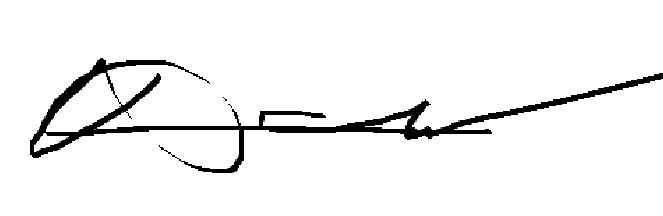
\includegraphics[height=1.5cm]{graphics/unterschrift_Leander.png} \\[0.1cm]
(Ort, Datum) & \hspace{0.3\linewidth} & (Unterschrift)
\end{tabular}
\end{center}
%\clearpage

\thispagestyle{empty}

{\LARGE\textsf{\textbf{Erklärung}}\bigskip}

% \typMeinerArbeit und \themaMeinerArbeit werden in config.tex definiert
%
Ich versichere hiermit, dass ich die vorliegende Arbeit mit dem Thema: \emph{\themaMeinerArbeit} selbstständig verfasst und keine anderen als die angegebenen Quellen und Hilfsmittel benutzt habe.
Ich versichere zudem, dass die eingereichte elektronische Fassung mit der gedruckten Fassung übereinstimmt.%


\vspace{3cm}

\begin{center}
\begin{tabular}{ccc}
(Ort, Datum) & \hspace{0.3\linewidth} & (Unterschrift)
\end{tabular}
\end{center}

%
\clearpage

\thispagestyle{empty}

{\LARGE\textsf{\textbf{Ehrenwörtliche Erklärung}}\bigskip}

% \typMeinerArbeit und \themaMeinerArbeit werden in config.tex definiert
%
Ich versichere hiermit, dass ich die vorliegende Arbeit mit dem Thema: \emph{\themaMeinerArbeit} selbstständig 
verfasst und keine anderen als die angegebenen Quellen und Hilfsmittel verwendet habe und diese Arbeit bei keiner 
anderen Prüfung mit gleichem oder vergleichbarem Inhalt vorgelegt habe und diese bislang nicht veröffentlicht wurde.
Des Weiteren versichere ich, dass die eingereichte elektronische Fassung mit der gedruckten Fassung übereinstimmt.%


\vspace{3cm}

\begin{center}
\begin{tabular}{ccc}
Glatten, \abgabeDatum & & 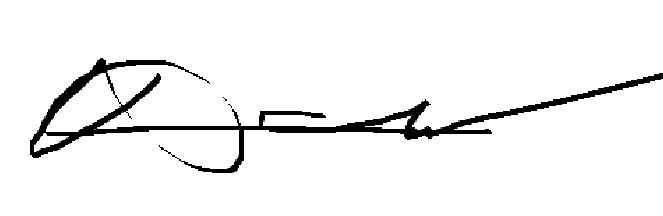
\includegraphics[height=1.5cm]{graphics/unterschrift_Leander.png} \\[0.1cm]
(Ort, Datum) & \hspace{0.3\linewidth} & (Unterschrift)
\end{tabular}
\end{center}
\end{document}
